\documentclass[11pt,a4paper,oneside]{article}

\usepackage{amssymb,amsmath}
\usepackage[T1]{fontenc}
\usepackage[utf8]{inputenc}
\usepackage{lmodern}
\usepackage{graphics}
\usepackage[english]{babel}
\usepackage{csquotes}
\usepackage{booktabs}
\usepackage{multirow}
%\usepackage[notes,backend=biber]{biblatex-chicago}
\usepackage{rotating}
\usepackage{threeparttable}
\usepackage{enumitem}
\usepackage[hang,flushmargin]{footmisc} 
\usepackage[a4paper,left=3.5cm,right=3.5cm,top=2.5cm,bottom=2.5cm]{geometry}

\renewcommand{\baselinestretch}{1.5}

\newenvironment{changemargin}[2]{%
  \begin{list}{}{%
    \setlength{\topsep}{0pt}%
    \setlength{\leftmargin}{#1}%
    \setlength{\rightmargin}{#2}%
    \setlength{\listparindent}{\parindent}%
    \setlength{\itemindent}{\parindent}%
    \setlength{\parsep}{\parskip}%
  }%
  \item[]}{\end{list}}


\begin{document}
\pagenumbering{gobble}
\begin{titlepage}
   \begin{center}
        \vspace*{1cm}
 
        \textbf{Can Machine Learning Improve\\Matching Quality\\ In Matching Estimator?}
     
        %\vspace{0.5cm}
            %Thesis Subtitl
     
        \vspace{1.5cm}
     
        Masterarbeit\\
        für die Prüfung zum Master of Science (M. Sc.) Economics\\
        eingereicht beim Prüfungsausschuss für den Masterstudiengang Economics\\
        der\\
        Fakultät für Wirtschafts- und Sozialwissenschaften\\
        Ruprecht-Karls-Universität Heidelberg\\
           
        \vspace{0.8cm}
 
        2019
        \vspace{2.5cm}
        \vfill
   \end{center}
   \textbf{Jongoh Kim}\\
    born in 16.04.1991
\end{titlepage}

\textbf{"Hiermit versichere ich, dass ich die vorliegende Arbeit selbstständig
und ohne unerlaubte fremde Hilfe verfasst habe und dass alle wörtlich
oder sinngemäß aus Veröffentlichungen entnommenen Stellen dieser
Arbeit unter Quellenangabe einzeln kenntlich gemacht sind."}

\newpage
\tableofcontents
\newpage
\pagenumbering{arabic}
\section{Introduction}
It wouldn't be an exaggeration to say the word "Machine Learning" is the one of the most fantasized terms in current times. It surely is an amazing technological advancement which deeply affects our daily lives today. Its application varies widley: simply from Google search to complicated artificial intelligence (A.I). 
\par
However, as Athey (2018)\cite{athey2018impact} mentions, the definition of machine learning is not clearly established. To loosely define machine learning, it is a group of statistical methods and computation algorithms to maximize the accuracy of predicting potential outcomes. As machine learning methods do make accurate predictions on various types of problems (regression, classification,  etc.), machine learning methods are being applied to numerous fields: medicine, marketing, and also economics.
\par
Some economic papers exist which explain what machine learning is, and how it could be applied to economic research. Athey(2018)\cite{athey2018impact} provides a concise  but extensive overview of machine learning in the academic field of economics. It explains what machine learning is; what  different types of machine learning exist (unsupervised, supervised, etc.) to which academic questions machine learning could provide an answer; and what the future impact of machine learning in economic research could be. Mullainathan \& Spiess (2017), focus more on a single type of machine learning, supervised machine learning, and on practical issues if a researcher is implementing machine learning. The paper clearly explains how machine learning works by showing a few examples of how machine learning would be used in an economic research. Also, it mentions several key points a researcher would be curious about, for example, which method of machine learning is appropriate for a given research project. Both papers, however, agree that machine learning could be applied in matching estimator method by calculating propensity scores.
\par
Several papers have already tried to explore the potential of implementing machine learning methods in academic research. Lee et al. (2010)\cite{lee2010improving} finds out that a boosted classification tree performs well in propensity score weighting but with simulated data in a medical context. Cannas and Arpino (2019)\cite{cannas2019comparison} finds the performance of Random Forest is better than other statistical methods in propensity score matching and propensity score weighting, using the identical specifications as Lee et al. (2010).\cite{lee2010improving} 
\par
On the other hand, Brown et al.(2018)\cite{brown2018estimating} argues LASSO (Least Absolute Shrinkage and Selection Operator), Boosting, and Deep Learning outperform Random Forest at least in the Cox Proportional Hazard Model. Also, Goller et al.(2019)\cite{goller2019does} concludes LASSO based logistic regression performs better than other models in propensity score matching. However, the paper uses a radius matching framework, which is different from this paper. In addition, the paper argues that Random Forest epecially results in subpar performance when treatment share is low. To summarize, no clear conclusion exists whether implementing machine learning methods in propensity score matching results in better performance, in terms of matching quality, than traditional statistical models.
\par
Hence, I seek to shed more light on this research question by implementing four different machine learning models to calculate propensity scores for matching. The four machine learning methods applied in this study are linear SVM, Radial SVM, Random Forest, and XGBoost. Two variations of SVM models are used since they are one of the classical machine learning methods for classification problems and since SVM model is closely related to LASSO (Jaggi, 2013)\cite{jaggi2013equivalence} and Logit model(Koller et al., 2007, p357).\cite{koller2007introduction} For comparison, the traditional Logit model is also used to calculate propensity scores. 
\par
The setting of this paper is minimum wage introduction in west Germany. The paper partially investigates whether minimum wage introduction in west Germany has affected the capital-labor ratio.\footnote{It is the total value of fixed asset divided by total number of employees in a firm} The value of interest is the average treated effect of the treated (ATT) of minimum wage introduction on the capital-labor ratio of a firm. Note that the scope of this study is restricted to the Nursing and Caring sector, not the whole economy, for the purpose of simplicity. Also, it is because the main focus of this study is to examine the matching quality generated by machine learning methods, not to obtain an overall measure of the impact of minimum wage introduction on a firm's capital-labor ratio in west Germany. 
\par
The dataset used for calculating propensity scores is a dataset which includes extensive data from firms located in west Germany. It includes 1,259,312 observations with a time window from 2007 to 2014. The dataset has lots of information from firms: financial information, in which industry a firm is operating, the company type, and etc. In addition, most importantly, it also tells us whether a firm has had a minimum wage.
\par
After propensity scores are generated by five various statistical models with a detailed dataset of firms in west Germany, nearest neighbor matching is applied to produce a matched dataset. With resulting matched datasets,  the matching quality of each dataset is measured using standardized difference in means of propensity scores and the variance ratio of propensity scores between the treated group and the control group. 
\par
To check whether treatment share or relative size of the number of observations in the control group affects the outcome, a bigger size of the control group is used as a robustness check. The same analytical process is done on the larger control group. More details will be discussed in section 4. 
\par
The paper is structured as follows. In section 2, I will explain briefly what a machine learning is and provide the theoretical background of each machine learning method implemented in this study. Section 3 describes which data has been used for the analysis. In section 4, I will explain in detail how the matching procedure is done in my analysis. Section 5 provides the results of this study: generated matching quality by each statistical model and estimated ATT of minimum wage introduction on a frim's capital-labor ratio. Lastly, a discussion and conclusion are included in section 6 and 7.
%============================================================================================
%============================================================================================
%============================================================================================
\section{Common Machine Learning Methods}
In this section, I introduce machine learning methods which are commonly used in classification problems. The methods will be implemented later to calculate propensity scores for matching. With the propensity scores generated by machine learning methods and by traditional logistic regression, I will compare the matching quality later in section 4. I have borrowed most of the concepts, figures, and equations to explain machine learning methods from the book \emph{An Introduction to Statistical Learning} (Koller et al., 2007).\cite{koller2007introduction} Thus, for a more detailed explanation, please refer to the book.

\subsection{Machine Learning (ML)}
What is machine learning? As Athey points out in her paper (2018)\cite{athey2018impact}, it is surprisingly difficult to define what machine learning is. I only slightly adjust the definition of machine learning from Athey (2018)\cite{athey2018impact} and define machine learning as: \emph{"a field that develops algorithms designed to be applied to datasets, with the main areas of focus being prediction ... ."}. As the definition states, the main objective of machine learning is to accurately predict various types of outcomes: continuous (regression), discrete (classification), and unknown (clustering). 
\par
Machine learning could be split into two large blocks: supervised learning and unsupervised learning. The name "supervised" comes from the fact that supervised machine learning trains its model by knowing what the measurable aspects (covariates or features\footnote{The expressions, covariates and features, will be used interchangably.}) and the right outcomes of observations are. It is as if a researcher is supervising the machine's learning process. On the other hand, unsupervised learning models have limited information on each observation, especially in a sense that no outcome variable is provided. Hence, unsupervised learning is generally used in cases when it is typically difficult to measure outcomes or the data is unstructured, such as pictures, texts, and videos. Unsupervised learning aims to group similar observations based on their features. On the contrary, supervised learning is applied in datasets which provide measurable covariates and outcomes: the typical type of datasets mostly used in economic studies. As the dataset used in this study is also suitable for supervised learning and supevised learning methods are used in my analysis, I will proceed by explaining more about machine learning by narrowing its scope to supervised learning.
\par
Supervised machine learning can be again divided into two segments: parametric and non-parametric. Parametric machine learning methods have their own functional forms to predict outcomes. Non-parametric machine learning methods, however, have no pre-defined mathematical form to build a model. One prominent example of a parametric machine learning method in classification problems is the Support Vector Machine (SVM) method, and the one in non-parametric methods is the Tree method. Both of them are used in my analysis, and I implement two different versions of each method. Among different adaptations of SVM, linear SVM and radial SVM are used, and Random Forest and XGBoost are used as one of the many variations of the Tree method. A more comprehensive explanation follows in the subsequent subsections.
\par
Most of the time, good machine learning models are built so that they can obtain precise predictions when a realized outcome is not yet available. Therefore, in general, a dataset would be split into two parts: a training set and a test set.  Machine learning models would typically build up a model with a training set, and its performance would be tested on a test set. A model which has the best performance in predicting outcomes in the test set would be chosen. The process of choosing which is the best machine learning model is done in this way so that researchers avoid choosing poor machine learning models which have over-fitted in a training set but generate low predicting power in a test get. As a result, researchers could have accurate out-of-sample predictions.
\par
However, the objective of constructing a machine learning model in this study is different from general cases. The models presented in this paper focuses on acquiring accurate propensity scores. It is distinct from generic settings in the sense that the main goal of the machine learning models is to have high accuracy in predicting in-sample outcomes, introducing minimum wage, and not to have precise predictions on out-of-sample observations. Hence, throughout this paper, no difference exists between a training set and a test set, and both of them are the whole dataset.

\begin{table}[t!]
	\centering
	\caption{Summary of Implemented Machine Learning(ML) Methods}
	\def\arraystretch{0.7}
	\begin{tabular}{*5c} 
		\toprule {} & \multicolumn{4}{c}{Supervised Machine Learning}\\
		{} & \multicolumn{2}{c}{Parametric ML} & \multicolumn{2}{c}{Non-parametric ML}\\
		\hline
		{} & \multicolumn{2}{c}{SVM} & \multicolumn{2}{c}{Tree}\\
		\midrule \multicolumn{1}{l|}{Characteristic} & \multicolumn{1}{r}{Linear} &\multicolumn{1}{r}{Non-linear} &\multicolumn{1}{r}{Bagging} &\multicolumn{1}{r}{Boosting}\\
		\multicolumn{1}{l|}{ML method} & \multicolumn{1}{r}{Linear SVM} &\multicolumn{1}{r}{Radial SVM} &\multicolumn{1}{r}{Random Forest} &\multicolumn{1}{r}{XGBoost}\\
	\end{tabular}
	\label{table:1}
\end{table}
%============================================================================================

\subsection{Support Vector Machine(SVM)}
The Support Vector Machine (SVM) method was firstly introduced by Cortes \& Vapnik (1995).\cite{cortes1995support} To provide a clear overview of how SVM works, it is necessary to talk about primitive forms of SVM: Maximal Margin Classifier (MMC) and Support Vector Classifier (SVC). 
\subsubsection{Maximal Margin Classifier (MMC)}
The approach of the Maximal Margin Classifier (MMC) method to classification problems is simple: finding a hyperplane in an $N$-dimensional space which can divide observations into 2 categories. For simplicity, I will explain further about SVM in a 2-dimensional space with covariates $X_{1}$ \& $X_{2}$ and an outcome variable $Y$ which could have a value of either one or negative one. 
\par
An ideal case of classification problems would be if a person could draw a line in two dimensional space which could work as a borderline distinguishing observations with outcome $y_{i}=1$ from observations with outcome $y_{i}=-1$. The line is a solution of the classification problem as it perfectly classifies observations with $y_{i}=-1$ and $y_{i}=1$. Let the separating hyper plane be:
\begin{align}
    & (\beta_{0}+\beta_{1}x_{i1}+\beta_{2}x_{i2}) = 0 \;\;\; \text{and,}\\
    & (\beta_{0}+\beta_{1}x_{i1}+\beta_{2}x_{i2}) > 0 \;\;if\; y_{i} = 1\\
    & (\beta_{0}+\beta_{1}x_{i1}+\beta_{2}x_{i2}) < 0 \;\;if\; y_{i} = -1
\end{align}
\par
However, the problem arises from the fact that there are an infinite number of lines which could classify observations perfectly as in Figure 1.\footnote{Left-hand panel of figure 9.2 on page 340 of the book Koller et al. (2007)\cite{koller2007introduction}} Thus, a standard is required to choose which line, or a hyperplane in higher dimensions, is the "best" classifier. As the name implies, MMC chooses the "best" classifier which has the maximum value of "margin." Margin is defined as the minimum  distance between the hyperplane and observations. Hence, MMC chooses a hyperplane which creates the biggest buffer space between two different classes.

\begin{figure}[t!]
    \centering
    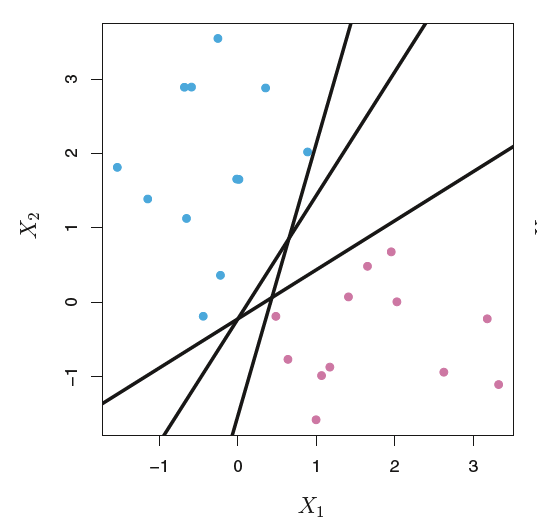
\includegraphics[scale = 0.5]{Figures/figure1.png}
    \caption{Multiple Separating Hyperplanes}
    \label{fig:figure1}
\end{figure}

\par
To explain MMC in a mathematical way, it is the solution to an optimization problem.
\begin{align}
	&\underset{\beta_{0}, \beta_{1}, \beta_{2}}{\text{maximize}}\; M\\
	&\text{subject to }\sum^{2}_{j=1}\beta^{2}_{j}\;=\;1\\
	&y_{i}(\beta_{0}+\beta_{1}x_{i1}+\beta_{2}x_{i2}) \; \geq\; M\;\; \forall i\; =\; 1,...,n
\end{align}
The problem is a two dimensional case with $n$ observations and it can be easily generalized to $N\in R_{+}$ dimensional space. Due to equation (2) and (3), an observation must have a positive value in $y_{i}(\beta_{0}+\beta_{1}x_{i1}+\beta_{2}x_{i2})$ if such a separating hyperplane exists, which perfectly classifies observations. Adding equation (5) and (6) to the previous fact, an observation must have a distance more than $M$, given that it has a positive value. It is because $y_{i}(\beta_{0}+\beta_{1}x_{i1}+\beta_{2}x_{i2})$ is the distance of an observation to the separating hyperplane. Thus, equation(4), (5), and (6) combined find a hyperplane which perfectly classfies observations, and maximizes the minimum distance between the hyperplane and observations: maximal margin classifier.
\par
As some people have already noticed, MMC heavily relies on a subset of observations which are near to the separating hyperplane, if one exists. In other words, observations which could be clearly distinguished or are far away from the separating hyperplane have not much importance in MMC. This is due to the fact that $M$ is the critical value in MMC and $M$ is calculated by a few observations which are closest to the hyperplane. These observations are called "support vectors." This is because 1) each observation is a vector and 2) these vectors "support" the hyperplane with maximal margin as the hyperplane would change even if support vectors slightly change. 
%\par
%It is not difficult to deduce why a hyperplane with maximal margin is considered the "best" classifier. A hyperplane with maximal margin is more robust to new observations than other hyperplanes with less margin. Imagine, a new observation enters into an existing two dimensional dataset which you have already used to generate a separating hyperplane with maximal margin. The separating hyperplane cuts through the the whole space leaving buffer zones to either classes with identical margin. As the separating hyperplane is chosen with maximal margin, it is less probable for the new observation to located on the wrong side of the hyperplane than hyperplanes with less margin. Thus, the criteria of choosing the separating hyperplane in MMC results in more robust classification.
\par
Unfortunately, it is highly unlikely a dataset exists to which MMC could be applied. As I have implied before, a dataset must be linearly separable to implement MMC. If no separating hyperplane exists which could perfectly classify observations into their right class, MMC cannot be used.
\subsubsection{Support Vector Classifier (SVC)}
To overcome the aforementioned problem, Support Vector Classifier (SVC) was introduced. In SVC, a dataset does not have to be perfectly linearly separable, which is the most attractive characteristics of SVC. SVC aims to correctly classify the majority of observations. Hence, SVC allows the separating hyperplane to misclassify some observations with a penalty. 
\par
SVC is the solution to a slightly different of the optimiziation problem from MMC.
\begin{align}
	&\underset{\beta_{0}, ..., \beta_{2}, \epsilon_{1}, \epsilon_{2}}{\text{maximize}}\; M\\
	&\text{subject to }\sum^{2}_{j=1}\beta^{2}_{j}\;=\;1,\\
	&y_{i}(\beta_{0}+\beta_{1}x_{i1}+\beta_{2}x_{i2}) \; \geq\; M(1-\epsilon_{i}),\\
	&\epsilon_{i} \geq 0, \;\;\; \sum^{2}_{i=1}\epsilon_{i}\leq C \;\;\text{where } C\geq0 
\end{align}
\par
$\epsilon_{i}$ is a so-called slack variable. If an observation lies on the wrong side of the hyperplane, it would have a value greater than one. A slack variable will have a positive value less than one if an observation lies on the right side of the hyperplane but has a distance less than the margin. A slack variable has a value of zero if an observation lies on the right side of the hyperplane and has a distance greater than or equal to the margin.
\par
$C$ is a tuning parameter which determines how many observations can have a distance less than the margin, violate the margin (and how severe is the violation), whether or not the observation is on the wrong side of the hyperplane. It is clearly stated in equation (10). The total sum of slacking variables must be less than or equal to $C$. Thus, if $C$ has a comparatively small value, less observations are allowed to violate the margin and the violations must be relatively moderate. 
\par
Most importantly, the value of $C$ is the critical value which significantly affects the bias-variance trade-off in SVC. If $C$ is large, SVC has high bias but low variance. SVC has low bias but high variance if $C$ is comparatively small.
\begin{figure}[t!]
    \centering
    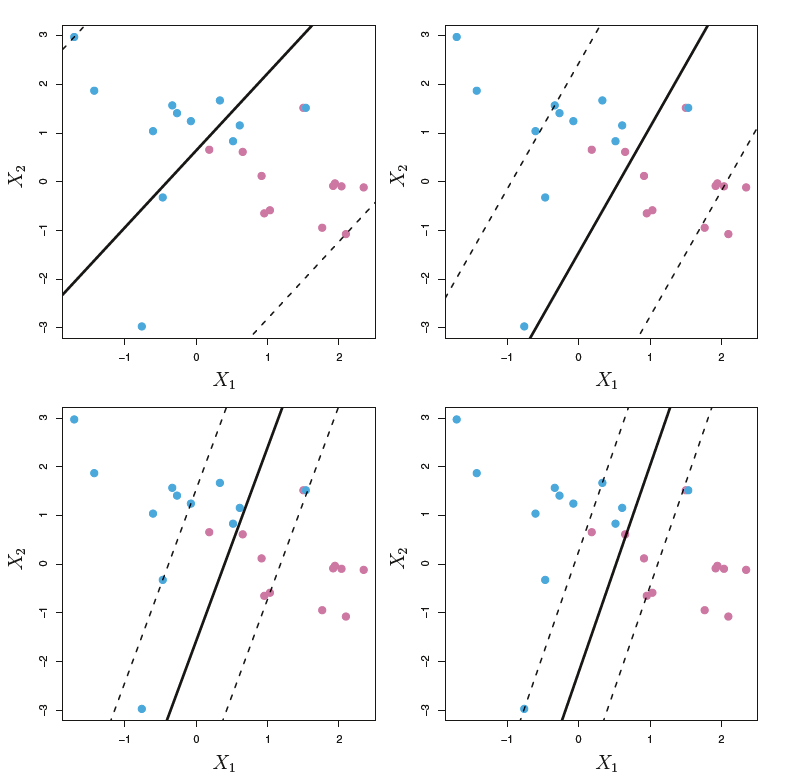
\includegraphics[scale = 0.5]{Figures/figure2.png}
    \caption{The role of the Tuning Parameter C}
    \label{fig:figure2}
\end{figure}

\par
The role of $C$ is best summarized in Figure 2.\footnote{Figure 9.7 on page 348 of the book Koller et al. (2007)\cite{koller2007introduction}} $C$ has the largest value in the upper left graph and the smallest value in the lower right. The upper right graph has a larger value of $C$ than the lower left. The straight line in each graph is the SVC and two dotted lines next to it show how big the margin is. As shown in the figure, with bigger $C$, there are more observations which are violating the margin or even on the wrong side of the hyperplane. On the other hand, less observations violate the margin or are located on the wrong side of the hyperplane when $C$ is relatively small. For example, on the top left panel, most of the observations are violating the margin and 5 blue dots are on the wrong side of the hyperplane. However, in the lower right graph, less than 10 observations violate the margin, and only three observations are on the wrong side of the hyperplane.

\subsubsection{Support Vector Machine(SVM)}
Although SVC allows some flexibility by allowing some observations to violate the margin, we are still restricted to the world of linearity. Support Vector Machine (SVM) lets us enter the realm of non-linearity. 
\par
It is necessary to mention the solution to the optimization problem from SVC before I explain how SVM allows non-linearity. I will not explain in detail how the solution is derived as it is too technical and not in the scope of this paper. The solution function can be written as:
\begin{align}
    f(x) = \beta{_0} + \sum_{i\in S}\alpha_{i}<x_{i}, x_{i'}>,
\end{align}
where $S$ is a set of support vectors, and $<x_{i}, x_{i'}>$ is an inner product of $x_{i}$ and $x_{i'}$: $\sum^{2}_{j=1}x_{ij}x_{i'j}$. The essential part of the solution function is the inner product. 
\par
SVM comes from generalizing the inner product part in SVC solution function, equation (11). If we generalize the inner product part into a function $K(x_{i}, x_{i'})$, the solution function is as follows.
\begin{align}
    f(x) = \beta{_0} + \sum_{i\in S}\alpha_{i}K(x_{i}, x_{i'}),
\end{align}
The function $K$ is a function often called a "kernel". If we set $K(x_{i}, x_{i'}) = \sum^{2}_{j=1}x_{ij}x_{i'j}$, then the solution function is as same as from SVC, and it is often called \emph{linear} SVM. However, the kernel can be set to a non-linear function. For instance, the most popular example of a ßnon-linear kernel function is the radial kernel function, and the corresponding SVM is called \emph{radial} SVM. The radial function has a form,
\begin{align}
    K(x_{i}, x_{i'}) = \text{exp}(-\gamma\sum^{2}_{j=1}(x_{ij}-x_{i'j})^{2}).
\end{align}
Hence, SVM can have a non-linear solution and could be applied to more general cases when a linear hyperplane cannot effectively classify observations as in figure 3.\footnote{Right-hand panel of figure 9.9 on page 353 of the book Koller et al. (2007)\cite{koller2007introduction}}
\begin{figure}[t!]
    \centering
    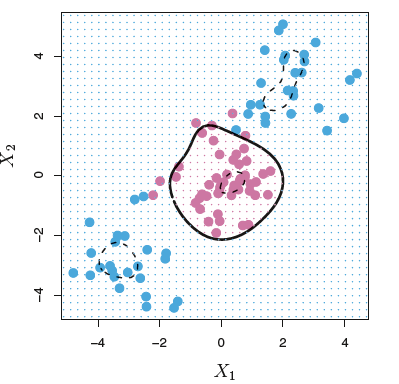
\includegraphics[scale = 0.5]{Figures/figure3.png}
    \caption{An Example of Raidal SVM}
    \label{fig:figure3}
\end{figure}
%============================================================================================
\subsection{Classification Tree}
Another popular machine learning method for solving classification problems is the classification tree method.\footnote{The term 'tree method' will be often used throughout this paper and it strictly stands for classification tree, not regression tree as this study focuses on a classification problem.} I will proceed explaining how the classification tree method works by again providing a two dimensional example. Then, I will state what are the pros and cons of the tree method, and how the method could improve its accuracy by implementing bagging and boosting. 
\par
Generally speaking, tree method solves classification problems by stratifying the feature, or covariate, space. A typical example is like in Figure 4.\footnote{Lower right panel of figure 8.7 on page 315 of the book Koller et al. (2007)\cite{koller2007introduction}} The tree method firstly divides the the feature space into two parts with a criterion: $X_{1}\leq-1$. Then, another split will be done on the region $X_{1}>-1$, depending on whether the value of $X_{2}$ is bigger than one. As a result, tree method perfectly classifies observations from green to yellow. 
\begin{figure}[t!]
    \centering
    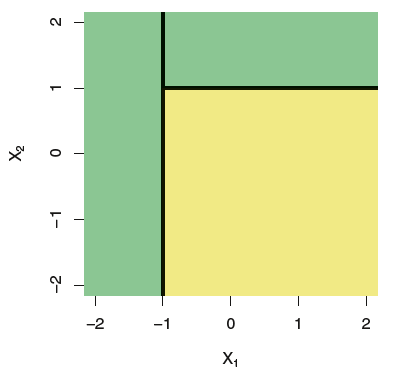
\includegraphics[scale = 0.7]{Figures/figure4.png}
    \caption{An Ideal Example of Implementing Classification Tree}
    \label{fig:figure4}
\end{figure}
\par
To explain in more detail, the tree method uses the so-called greedy algorithm to choose the next split. Such an algorithm is used to substantially decrease necessary computational power to decide the next split. In theory, it is best to consider all possible splits in all steps and choose the optimal split choices. However, an infinite amount of possible split choices exists, and it is almost impossible to consider all of them. Hence, in general, the tree method chooses the optimal split which can be done at each step, which is the essence of the greedy algorithm.
\par
In the classification problem, the optimal split is chosen which results in the minimum classification error rate. Classification error rate is simply the fraction of the number of least-occurring class observations by the number of total observations in a split. For example, let's say 10 observations exists in the region $X_{1}>-1$ in figure 4. Among the ten, eight observations are yellow, and two are green. Then, the classification error rate of the region would be $2 / 10 = 0.2$. Such a criterion is applied to the tree method because the tree method predicts classes depending on the most occurring class in a region. Using the same example, the tree method will predict observations which has an $X_{1}$ value higher than -1 as yellow with 20\% classification error rate.
\par
\begin{figure}[!t]
    \centering
    
\includegraphics[width=0.7\columnwidth]{Figures/cart.png}
    \caption{A Classification Tree}
    \label{fig:5}
\end{figure}
The advantage of using a simple tree method is that it is easy to interpret its result. For instance, look at figure 5(Brownlee, 2019).\cite{brownlee} Two features, weight and height, exist to determine whether an individual is a male or a female. The first split is done depending on whether an observation has a height higher than 180cm. This means the height criterion results in the lowest classification error rate in the whole dataset, and, of course, the height covarite plays more important role in predicting the sex of an observation than the weight covariate. Next, among observations who are shorter than 180cm, splitting the observations depending on their weight produces high prediction rate when the standard weight is set to 80kg. 
\begin{figure}[!t]
    \centering
    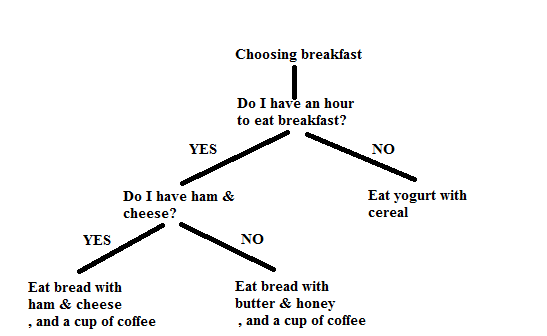
\includegraphics[width=0.8\columnwidth]{Figures/cart2.png}
    \caption{A Classification Tree}
    \label{fig:5}
\end{figure}
\par
Another benefit of using the tree method is that it resembles human decision making process. A simple example is shown in figure 6. Figure 6 illustrates a simplified version of my decision making process in a morning. First, I will check whether I have enough time to have a proper breakfast. If not, I will have a simple breakfast with a bowl of yogurt and some cereals in it. I won't make coffee and have a take-out on my way to university. If I have more than an hour for my breakfast time, I will firstly brew my espresso in a mocha machine, and look inside my fridge whether I have cheese and ham to eat with some bread. If I do have cheese and ham, I will have them with some bread slices. If I do not have any, I will eat some bread with butter and honey spread on them.
\par
However, tree method suffers from high variance problem. It is not difficult to deduce why a simple classification tree method has high variance. Tree is grown on a dataset making splits which results in lowest classification error at each step. When the model is tested on a new dataset, it is highly likely the model cannot predict the outcomes accurately unless the test set is substantially similar to the training set. If a tree is grown using the test set, the resulting tree might have large difference between the tree trained by using the training set. 
\par
As a result, the performance of a simple classification tree method in predicting outcomes is not as good as other statistical methods. Fortunately, predicting power of classification tree method can be significantly improved after bagging or boosting methods are applied. Random Forest is one of the most famous tree models which bagging method is implemented, and XGBoost is currently the most popular and the most powerful tree models with boosting. I explain each model and each method in subsequent subsections.

\subsubsection{Bagging}
The procedure of bagging is as follows. (1) Sample is bootstrapped, and multiple subsample are generated. (2) For each subsample, a tree is trained, or grown. (3) Then, the various resulting trees are averaged into one model. By applying the bagging method, tree methods could alleviate its high variance problem, and also increase its predicting power. The most popular tree model with bagging is the Random Forest method.
\\
\\
$\bullet$ Random Forest\\
The Random Forest method is a variation of the tree method applying the bagging method. The name "Random Forest" was coined by Leo Breiman in his 2001 paper: "Random Forests".\cite{breiman2001random} The model is an extension of Tin Kam Ho's original idea(1995)\cite{ho1995random}, and the algorithm designed by Breiman is still popular today.
\par
The name Random Forest is the perfect depiction of this tree model. Random Forest does apply bagging method, hence the model grows multiple trees: forming a forest. One important distinction from normal bagging process is that the model does not use same covariates to grow a tree in a subsample. Random Forest randomly chooses a subset of covariates to generate a tree in a subsample. The number of covariates to randomly choose in each subsample is the most important tuning parameter in the model, and the sqaured value of the total number of covariates is generally chosen(Koller et al., 2007)\cite{koller2007introduction} The reason why a subsample of covariates are chosen randomly is that to avoid growing similar trees in the bagging process. Imagine, if only few features play important role in predicting a class, then, during the bagging process, similar trees will be grown on each subsample because the few covariates play a significant role in generating low classification error rate. In such cases, the bagging process is not be effective. 
\par
The Random Forest model predicts the class of an observation by the majority of "votes". A "vote" is a predicted outcome of a tree. Hence, if we use Random Forest method by growing 100 trees in the bagging process, there will be 100 votes. The Random Forest method chooses the most popular vote among the votes, and predicts the class of an observation. Moreover, probability is simply the share of the votes casted to an according class among the total votes. If 30 trees voted an observation $a$ belongs to class 1, and the other 70 trees voted the observation is class 0, then the probability of the observation being class 1 is 30\%.

\subsubsection{Boosting}
The boosting method shares a similarity with the bagging process since boosting also relies on bootstrapped subsamples. However, if the bagging method focuses on growing $N$ trees independently on $N$ subsamples, the boosting method grows $N$ trees consecutively. The main idea of boosting is you learn from mistakes. 
\par
For simplicity, let's say, $N=2$. Then, a tree will grow on a first subsample ($N_{1}$) with $d$ number of splits. The resulting tree is $T_{1}$ but the final tree grown from $N_{1}$ is multiplying $T_{1}$ with $\lambda$, the learning rate. $\lambda T_{1}$ will most probably make some errors in predicting observations' classes. The next tree $T_{2}$ will set the error generated from $\lambda T_{1}$ as the main outcome variable and be trained, to minimize classification error rate. The resulting model is constructed by adding the previous final tree to recently grown $T_{2}$, but again multiplied by $\lambda$: $\lambda T_{2} + \lambda T_{1}$. If $N=3$, the final model would be $\lambda T_{3} + \lambda T_{2} + \lambda T_{1}$.
\par
The three major tuning parameters in the boosting method are $N$, $d$, and $\lambda$. Unlike bagging, boosting tends to overfit to a training sample when $N$ is large. Hence, it is important to create proper numbers of bootstrapped samples. $d$ controls the depth of each tree growing in a subsample $N_{i}$. According to \emph{Introduction to Statistical learning}(Koller et al., 2007)\cite{koller2007introduction}, the boosting tree model generally performs well when $d=1$. The learning rate, $\lambda$, is the weight attached to previously grown trees. In intuitive words, how much a model should learn from past models. As smaller the value of $\lambda$ is, the boosting tree model needs more time to train the model when $N$ is fixed.
\\\\
$\bullet$ XGBoost(XGB)\\
The XGBoost method is an advanced version of the boosting tree model, and developed by Tianqi Chen (2016).\cite{chen2016xgboost} Its name is an abbreviation of Extreme Gradient Boosting. Gradient boosting is a type of boosting algorithm initially designed by Jerome H. Friedman(2001).\cite{friedman2001greedy} The term, extreme, is attached to gradient boosting as XGBoost it has multiple advantages than existing gradient boosting tree model.
\par
Among various advantages, two stand out. First, it has an innate regularization process to avoid overfitting problem. The XGBoost model uses both LASSO and Ridge regression for the regularization process. Lastly, different from other traditional boosting methods, it grows trees in \emph{parallel} manner, not sequentially. This difference yields considerable improvement in computation time. According to a comprehensive comparison study by Pafka(2019)\cite{pafka}, when $\lambda=0.1$, $d=6$, $N=300$, and 10 million observations exist in a dataset, a gradient boosting tree model needs 5000 seconds to train. However, XGBoost requires a fifth of the time needed by gradient boosting tree model: 1000 seconds.
%============================================================================================
%============================================================================================
%============================================================================================

\section{Data}
The dataset used in my analysis is a modified version of data from Gathmann et al.(2018).\cite{Gathmann2018} The original data is firm-level data provided by Burea van Dijk (BvD). Its data primitively comes from Creditreform, the largest credit rating agency in Germany. The agency collects detailed data of active companies in Germany. A firm is classified to be economically active if (1) the firm is officially registered, or (2) the media mentions the firm or information of the firm's credit rating has been at least once requested by someone. The dataset contains numerous information of firms. Details include location of a firm, number of employees, firm's financial status, legal form of a company (AG, GmbH, and etc.), starting \& closing date of a firm, and more. More importantly, the dataset shows to which industry each firm belongs. 
\par
In the dataset, an industry code are attached to each firm with a length of two or four, under the Classification of Economic Activities, Edition 2008 (WZ2008). According to a report written by Federal Statistical Office Germany (2008)\cite{BundesamtClassification}, under the WZ2008 system there are 21 'sections', 88 'divisions', 272 'groups', 615 'classes', and 839 'sub-classes'. To provide a simple example, in section A (Agriculture, Forestry and Fishing), three divisions exist: Crop and animal production, hunting and related service activities; Forestry and logging; and Fishing and aquaculture. The industry code of the three divisions varies according to which scope a person is interested in. For sections, no specific industry code exists but labeled into capital alphabets, and industry codes for divisions are in two digit numbers, ranging from 01 to 99. The codes will be at maximum length of five when it is considered at the sub-class level. 
\par
Note that the analysis of this paper is focused on firms which falls under Nursing and Caring sector (Pflegebranche) and have been affected by the introduction of minimum wage. According to a report by Boockman et. al(2011)\cite{boockmann2011evaluation}, firms in Nursing and Caring sector have had minimum wage since August 2010 and minimum wage was between 7.5 euros and 8.5 euros when it was initially introduced. 
\par
Nursing and Caring sector is a term used in Germany's minimum wage law and does not align with WZ2008. Under the WZ2008 classification system, firms in section Q, Human Health and Social Work Activities, will have a two-digit industry code from 86 to 88, and Nursing and Caring sector falls under section Q. More specifically, the firms in Nursing and Caring sector will have either 87 or 88 two-digit industry code. However, not all firms with 87 or 88 industry code are in Nursing and Caring sector. Thus, some firms with 87 or 88 has not been affected by the introduction of minimum wage. To summarize, some firms in section Q with 87 or 88 are treated, and unaffected firms in section Q would have a two-digit industry code from 86 to 88.
\par 
Overall, two control groups exist throughout this paper. The first group\footnote{I would call it as 'local control group'} consists of firms which are in the same section Q but are not in Nursing and Caring sector. These firms, therefore, have an industry code in a range of 86 to 88 and have not experienced minimum wage introduction. The other group\footnote{This would be often referred as 'global control group'} comprises all firms in which no minimum wage was introduced, including also the firms in different sections. Hence, the firms would have an industry code ranging from 1 to 99.
\par
Most of the restrictions imposed on the dataset are set just to follow the similar steps as in Gathmann et al. (2018).\cite{Gathmann2018} To analyze the effect of minimum wage introduction, I restrict the time period as 3 years before and after minimum wage was introduced in Nursing and Caring sector in 2010. Hence, any firm has been removed from the dataset if a firm has a missing value in matching variables in a year or a firm does not have a full record between year 2007 and 2013. Also, certain sections were excluded from this dataset because no minimum wage was introduced in these sections, and their capital-labor structure and production process are distinguishably different from Nursing and Caring. The removed sections are section A (agriculture, forestry and fishing), K (financial and insurance activities), O (public administration and defence; compulsory social security), and R (arts, entertainment, and recreation). Also, I excluded any companies if their legal form is not either GmbH or GmbH \& Co. KG.\footnote{Less than 3\% of total observation falls into this category.} However, different from Gathmann et al. (2018)\cite{Gathmann2018}, I only focus on firms which are operating in west Germany. 
\par 
In the end, 3,794 and 134,860 firms exist for each year in the dataset.\footnote{These two datasets will be sometimes referred as "original" datasets, distinguishing from newly generated datasets in section four} The former is the number when the local control group is used as a control group. The latter happens if global control group is used for analysis. More detailed explanation of these two groups would be stated in subsection 4.1.2. In both cases, 1,846 treated firms exist. As the time period of my analysis is from 2007 to 2013, total observations are 26,558 and 944,020, respectively. 
%============================================================================================
%============================================================================================
%============================================================================================

\section{Empirical Approach}
\subsection{Matching procedure}
In brief, the matching procedure of my analysis is as the following. I consider observations from 2008, 2 years before the introduction of minimum wage in Nursing and Caring sector, for the matching. Generally, matching variables are as same as the ones used in Gathmann et al. (2018)\cite{Gathmann2018}: capital intensity\footnote{total fixed asset divided by total asset}, total liability in log value, log value of total asset, age of a firm in log value, and a dummy variable showing whether a firm is located in an urban area or not. I use four different machine learning methods and a traditional logistic regression to calculate propensity scores of each firm, which illustrate how a firm would likely to be affected by minimum wage introduction. Then, firms would be matched by the nearest neighbor matching method without replacement. 
%============================================================================================
\subsubsection{Training machine learning models}
As I have explained in section two, the importance of setting the tuning parameters in machine learning methods is paramount. It deeply affects the accuracy of a machine learning method's prediction, and, hence, heavily influences result of my analysis. Through out the whole paper, each machine learning method are trained to find the best super parameters which generate the highest accuracy. The training process is done by using the 'train()' function from an R package called 'caret'(Kuhn, 2008).\cite{JSSv028i05} The values of tuning parameter are equal regardless of which control group is used for analysis, which will be explained in further detail in coming subsection.
\par 
How the function trains machine learning models is as follows. The function, firstly, generates multiple possible values for the tuning parameters of corresponding machine learning method. For each possible value, the model is trained on little different data, and the function compares the performance of each trained model. As the focus of this paper is classification, the function measures the performance as how accurately a trained model predicts right class of an observation. Finally, the best values of tuning parameters are chosen which result in high accuracy in predicting outcomes with small variance.
%============================================================================================
\subsubsection{Setting control groups}
There are two types of control groups in my analysis: local control group and global control group. The former is constructed based on an assumption that only the firms in the same section are "similar" enough to be considered as a control group. However, it is also possible that other firms which are in different sections and which have not had minimum wage introduction could be considered as potential control group. Hence, my analysis, comparing the matching quality between traditional logistic regression and four different machine learning methods are done two times, each with a different control group. 1,947 firms are included in local control group, and global control group has 132,938 observations. 
\begin{table}[t!]
	\centering
	\caption{An Overview of Different Matching Qualities}
	\def\arraystretch{0.7}
	\begin{tabular}{*4c} 
		\toprule {} & \multicolumn{2}{c}{\underline{Control Group}} & \multirow{2}{*}{Methods}\\
		{} & Local & Global & \multirow{2}{*}{}\\
		\midrule \multirow{2}{*}{Same Matching Variables} & A1 & B1 & Logistic Regression\\
		\multirow{2}{*}{} & A2 & B2 & 4 machine learning Methods\\
		Different Matching Variables & A3 & B3 & Random Forest \& XGBoost		
	\end{tabular}
	\label{table:2}
\end{table}

\par
As a result, six different matching qualities are measured throughout this paper and these are well classified in Table 2. Results A1, A2, and A3 are derived from using firms in Nursing and Caring sector as the control group. On the other hand, B1, B2, and B3 are the results by putting all firms which did not have minimum wage, regardless of which sector they belong to, as the control group. The numbering comes from the difference in methods and matching variables. Both A1 and B1 are generated by conducting logistic regression by using the same default five matching variables which are mentioned in section 4.1. Same matching variables are utilized in A2 and B2 but four machine learning methods are implemented to calculate propensity scores for matching. A3 and B3 are results driven by feature selection process. Feature selection process is, simply speaking, a procedure choosing which covariates should be included in a machine learning model, depending on its importance. Thus, the matching variables in A3 and B3 are different from other results, and only Random Forest method and XGBoost method are chosen among other machine learning methods. More detailed description of the feature selection process of A3 and B3 will shortly follow in the next subsection.
%============================================================================================
\subsubsection{Matching variables}
It is not an exaggeration to say choosing matching variables is one of the most essential parts in matching procedure. To explore the full potential of implementing machine learning methods in matching, I give a variation in which matching variables are used in calculating propensity scores. In one part, I use same matching variables to calculate the propensity scores. In the other part, I let two non-parametric machine learning methods, Random Forest and XGBoost, to help me choose which matching variables I should use to calculate propensity scores depending on each variable's importance in predicting whether a firm would introduce minimum wage.
\par 
Firstly, I use same matching variables to calculate propensity scores but with different methods. The matching variables are capital intensity, log value of total liability , log value of total asset, log value of a firm's age, and an urban dummy variable showing whether a firm is located in an urban area. The reason why I firstly fix the matching variables to calculate propensity scores is to check whether machine learning methods would result in better matching quality than traditional methods when the only difference is which method is used to calculate propensity scores. I set the result from using logistic regression as my baseline result as it is one of the most widely used traditional methods to calculate propensity scores.
\par
Also, I calculate propensity scores by using different matching variables with Random Forest method and XGBoost method after feature selection process. Steps to choose appropriate matching variables are as follows. First, I generate a separate dataset just for the two machine learning methods, including all observations in the 7-year period. Then, I pick a list of variables which could have any slightest impact on a firm to introduce minimum wage. Initially, they were 27 variables but, after eliminating any variable which has missing values more than 30\% of total observation and any variable which has close-to-zero variance, for instance company type and solvency status, 14 variables remained: log value of total number of workers, log value of total asset, log value of capital asset, log value of intangible assets, log value of fixed asset, log value of current asset, log value of inventories, log value of total equity, log value of total liability, fixed asset to total asset ratio, total equity to total asset ratio, fixed asset to current asset ratio, log value of total inventory, log value of tangible asset, log value of current asset, log value of a firm's age, and a dummy variable indicating whether a firm is located in urban area or not. 
\par
Then, in case of local control group, missing values are imputed by using K nearest neighbor method (K=1). After the imputation process, I exclude all the observations which are not from year 2008 and are not included original dataset which I have mentioned at the end of section three so that the new dataset\footnote{"non-parametric dataset" will often exchangably used as the dataset is constructed for the two non-parametric machine learning methods: Random Forest \& XGBoost.} has the same observations as the original dataset. 
\par
For global control group, median imputation was for each firm was done due to computation limitation. Even after the imputation, some firms have missing values in log intangible assets and log inventroy values. Therefore, these two variables were removed and 12 variables remain in the non-paramteric dataset. Again, only observations in 2008 stay in the dataset and other observations are removed. 
\par
In addition, variables which have low importance in predicting whether a firm would be treated are ruled out. When local control group was used to train the two machine learning models, the urban dummy variable is excluded in both RF \& XGBoost as it has distinguishably less importance in predictions than other variables method. In case of RF, permuting the urban variable resulted in only a roughly 5\% point decrease in mean accuracy rate and approximately 17 decrease in mean Gini index.\footnote{It is another measure showing whether a variable has strong predicting power in a local sense. The higher the value of mean decrease of Gini index is, the according variable has a larger importance in locally predicting outcomes. Depending on this measure, each split is conducted.} On the contrary, the variable with second lowest mean decrease in accuracy has a value of approximately 8\% points in mean accuracy decrease but roughly 114 in mean decrease in Gini.\footnote{The second lowest value for mean decrease in Gini is from the variable capital intensity variable with a value of approximately 88.} Also, the urban variable played such a small roll in XGBoost as it is the only variable which results in less than 1\% points decrease in whole predicting power of the model when it is omitted.
\par
Overall, the new non-parametric datasets have 3,794 and 134,860 observations, depending on whether local or global control group is considered. Note that, few differences exist between the two non-paramteric datasets in terms of imputation process and which variables are included.
After matching process, 3,692 observations are remained in the matched dataset, regardless local or global control group is used. It is due to the fact that 1,876 observations are the treated firms in both cases.
%============================================================================================
%============================================================================================
%============================================================================================

\section{Result}
In this section, I explain the details of statistical models I have implemented in the analysis of this paper, make comparison between matching quality derived from traditional logistic regression and four different machine learning methods, and briefly explain the impact of minimum wage introduction on capital-labor ratio.\footnote{Fixed asset divided by the number of employees} Firstly, I show the specifics of the models, especially machine learning, in terms of what are the values of tuning parameters of each machine learning method after the training process. Then, I compare the resulting matching quality when local control group was used and the matching quality with global control group. Lastly, I will do a simple pooled OLS regression to measure the effect of minimum wage introduction on capital-labor ratio of firms.
%============================================================================================
%============================================================================================
\subsection{Model specifics}
Here, I explain the details of each statistical model employed through out this paper. Information I provide in this subsection is of machine learning methods after successfully trained. I will more focus on performances of logistic regression and four machine learning methods, rather than giving detailed description of each model's tuning parameters. Thorough explanation of the values of tuning parameters of each machine learning model is provided in Appendix section 1. The performance of every statistical model is summarized in table 3. 

\begin{table}[t!]
	\centering
	\caption{An Overview of Models' Performance}
	\begin{threeparttable}
	\def\arraystretch{0.7}
	\begin{tabular}{*5c} 
		\toprule 
		{} & \multicolumn{2}{c}{Local} & \multicolumn{2}{c}{Global}\\
		{Method} & {Accuracy} & {Variance} & {Accuracy} & {Variance}\\
		\midrule 
		\multicolumn{1}{l}{Logit} & \multicolumn{1}{r}{0.599} & \multicolumn{1}{r}{1.473} & \multicolumn{1}{r}{0.592} & \multicolumn{1}{r}{253.349}\\
		\multicolumn{1}{l}{Linear SVM} & \multicolumn{1}{r}{0.599} & \multicolumn{1}{r}{1.031} & \multicolumn{1}{r}{0.986} & \multicolumn{1}{r}{0.000}\\
		\multicolumn{1}{l}{Radial SVM} & \multicolumn{1}{r}{0.624} & \multicolumn{1}{r}{0.656} & \multicolumn{1}{r}{$\bullet$} & \multicolumn{1}{r}{$\bullet$}\\
		\multicolumn{1}{l}{Random Forest} & \multicolumn{1}{r}{0.612} & \multicolumn{1}{r}{0.775} & \multicolumn{1}{r}{$\bullet$} & \multicolumn{1}{r}{$\bullet$}\\
		\multicolumn{1}{l}{XGBoost} & \multicolumn{1}{r}{0.640} & \multicolumn{1}{r}{0.073} & \multicolumn{1}{r}{0.986} & \multicolumn{1}{r}{0.000}\\
		\multicolumn{1}{l}{\multirow{2}{*}{Random Forest}} & \multicolumn{1}{r}{\multirow{2}{*}{0.725}} & \multicolumn{1}{r}{\multirow{2}{*}{0.333}} & \multicolumn{1}{r}{\multirow{2}{*}{$\bullet$}} & \multicolumn{1}{r}{\multirow{2}{*}{$\bullet$}}\\
		\multicolumn{1}{l}{\multirow{2}{*}{after feature selection}} & \multicolumn{1}{r}{\multirow{2}{*}{}} & {}\\
		\multicolumn{1}{l}{\multirow{2}{*}{XGBoost}} & \multicolumn{1}{r}{\multirow{2}{*}{0.711}} & \multicolumn{1}{r}{\multirow{2}{*}{0.106}} & \multicolumn{1}{r}{0.986} & \multicolumn{1}{r}{0.000}\\
		\multicolumn{1}{l}{\multirow{2}{*}{after feature selection}} & \multicolumn{1}{r}{\multirow{2}{*}{}} & & \multicolumn{1}{r}{} & \multicolumn{1}{r}{}\\
		\\\bottomrule
	\end{tabular}
	\begin{tablenotes}[para,flushleft]
	    \linespread{1}\footnotesize
	    Note: The values of accuracy and variance is generated from 10-fold cross-validation. The accuracy column shows the mean value of accuracy from the cross-validation process. The variance of the ten accuracy values generated from the cross-validation process is shown in the variance column but multiplied by 1000.
	\end{tablenotes}
    \end{threeparttable}
	\label{table:3}
\end{table}


\par
Table 3 shows how accurately each model has predicted an observation in the training set would be treated. Note that the training set is the whole dataset, and it has different number of total observations, depending on whether local control group or global control group is used: 3,794 and 134,860 respectively. Hence, the treatment share in each case is roughly 49.45\% and 1.40\%. First and third column present the mean accuracy value of each model after 10-fold cross validation. Variance of the ten accuracy values of each machine learning model is listed in second and fourth column but multiplied by a thousand. The first two columns display performance of all statistical models when local control group is used. Performance of all methods using global control group is illustrated in third and fourth column.
\par
As I expected, all machine learning methods outperform the traditional Logit model in terms of accurate prediction. When local control group is used, logistic regression results in the lowest accuracy rate\footnote{Logit model has slightly lower accuracy rate than Linear SVM by approximately 0.03\% points} (59.9\%) and the highest variance of 1.473. Linear SVM model comes in as the second worst performing model with similar prediction rate as the Logit model but with rather slightly less variance (1.031). Radial SVM model performs a bit better than the Linear SVM . It accurately predicted 62.4\% of total observation's outcomes and has a variance of 0.656. The performance of Random Forest model is slightly better than Linear SVM model but worse than Radial SVM model. It has an prediction rate of 61.2\% and variance of 0.775. Among models with default five matching variables, XGBoost performed the best in both accuracy and variance. 

\par 
However, when feature selection process is implemented in both Random Forest model and XGBoost model, the Random Forest model has better accuracy than XGBoost. Its accuracy rate is 72.5\% whereas the accuracy rate of XGBoost model is 71.1\%. However, in terms of variance, XGBoost results in more stable prediction rate than the Random Forest model. The variance of the XGBoost model is 0.106, and Random Forest model has variance of 0.333. Note that these variance values are the values multiplied by 1000. If the values are once again divided by a thousand and squared to calculate the original values of standard deviation, the values are approximately 0.010 and 0.018, respectively. Hence, the range of XGBoost accuracy rate overlaps with the range of Random Forest accuracy rate. It is, therefore, difficult to assert which model is better than the other. Nevertheless, it is clear that Random Forest model and XGBoost model after feature selection outperform other models.

\par
If the control group is global control group, all three machine learning methods almost perfectly predicts the outcome. I believe it is due to the fact the treatment share is so low. Therefore, the three models could easily produce high accuracy rate even if they blindly predicts all observations to be non-treated. However, it is a mystery that Linear SVM model, nevertheless, predicts the majority of observations to be treated even if in raw data. In case of the traditional Logit model, its accuracy rate has even decreased, and the variance of 10-fold cross-validated accuracy has increased significantly, more than 170 times.
%============================================================================================
%============================================================================================
\subsection{Matching quality}
The matching procedure I have explained in section four relies on two essential assumptions. The first assumption is the conditional independence: conditioning on covariates, potential non-treated outcome is independent of treatment assignment, and the other assumption is that no deterministic covariate exists which could perfectly predict a firm would introduce minimum wage. 
\par 
The second assumption also implies that a substantial overlap should exist in propensity score distributions of the treatment group and the control group for a successful matching process. Hence, to check whether such an overlap exists, scatter plots of calculated propensity scores are presented and analyzed in this section.
\par
Moreover, a numerical diagnostic and a graphical diagnostic are examined to measure the quality of matching. The diagnostics are the standardized difference of means of the propensity score and the ratio of the variance of the propensity score in the treatment group and the control group. The two diagnostics measure whether the empirical distribution of covariates is similar in both the matched treated and the matched control, and are the two of three measurements presented in Rubin (2001)\cite{rubin2001using} for gauging the similarity in the two groups.
%============================================================================================
\subsubsection{Local control group}
\begin{figure}[!t]
    \minipage{0.5\textwidth}
  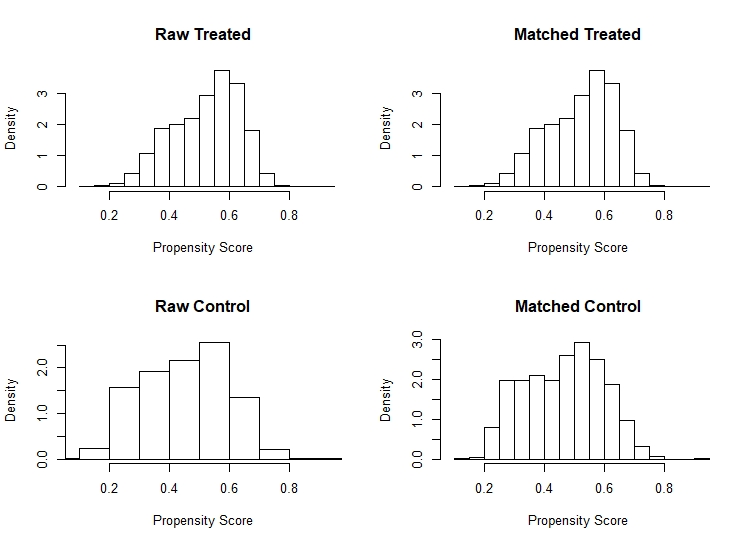
\includegraphics[width=\linewidth]{Figures/local_logit_hist.jpeg}
  \caption{Logit}\label{fig:histogram1}
\endminipage\hfill
\minipage{0.5\textwidth}
  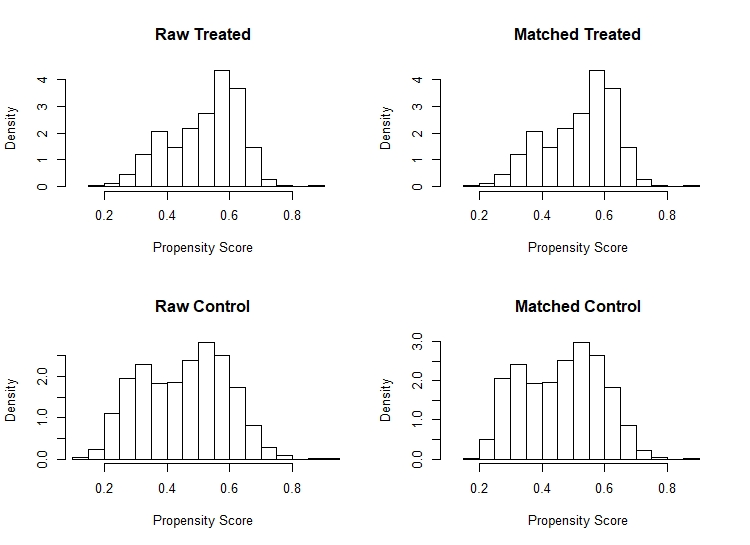
\includegraphics[width=\linewidth]{Figures/local_svm_hist.jpeg}
  \caption{Linear SVM}\label{fig:histogram2}
\endminipage\hfill
\minipage{0.5\textwidth}%
  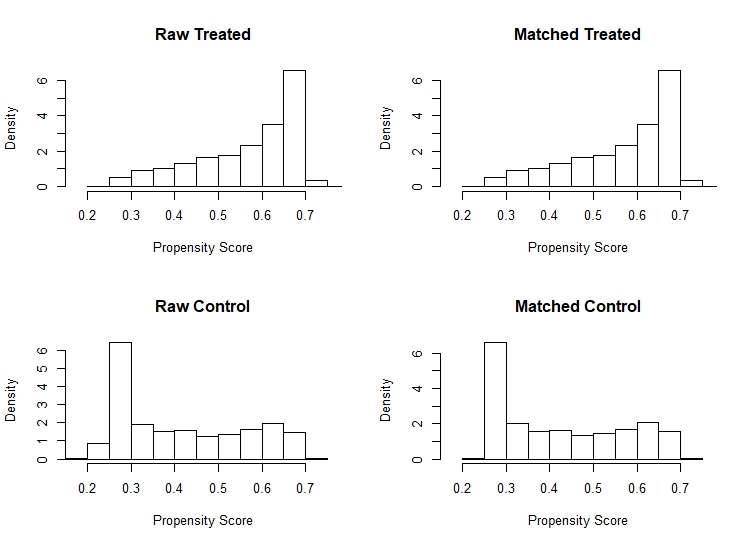
\includegraphics[width=\linewidth]{Figures/local_ksvm_hist.jpeg}
  \caption{Radial SVM}\label{fig:histogram3}
\endminipage\hfill
\minipage{0.5\textwidth}
  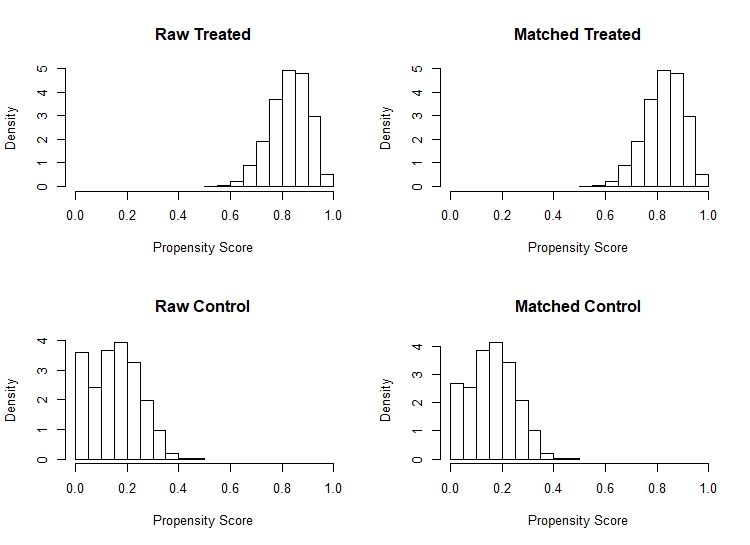
\includegraphics[width=\linewidth]{Figures/local_rf_hist.jpeg}
  \caption{Random Forest}\label{fig:histogram4}
\endminipage\hfill
\end{figure}
$\bullet$ \textbf{Region of Common Support}\\
The distribution of calculated propensity scores are shown in figure one to figure seven. The propensity scores are generated by using local control group. Note that I use nearest neighbor matching method. Therefore, it is ideal for me to have a distribution of matched control groups much similar to the distribution of the matched treated. 
\par 
However, half of the machine learning methods produce skewed distributions. In figure three, four, and six, most of the treated observations have high propensity scores, resulting in left skewed distribution. On the other hand, the majority of firms which have not introduced minimum wage have low propensity scores, and, thus, right skewed distributions are generated. At least in Radial SVM case (figure three), the distributions of the treated and the non-treated overlap each other. However, whenever Random Forest method is applied for calculating propensity scores, the resulting distributions of the propensity scores are so skewed to either end that no overlap exists.

\begin{figure}[!t]
    \minipage{0.5\textwidth}
        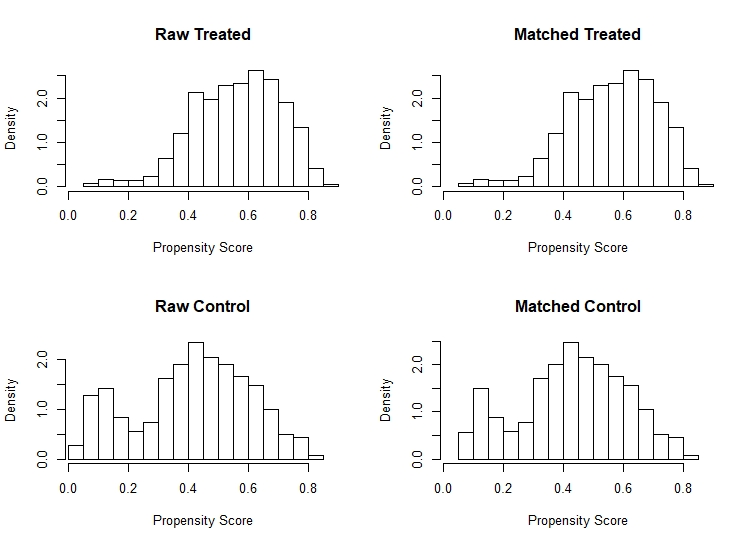
\includegraphics[width=\linewidth]{Figures/local_xgb_hist.jpeg}
        \caption{XGBoost}\label{fig:histogram5}
    \endminipage\hfill
    \minipage{0.5\textwidth}%
        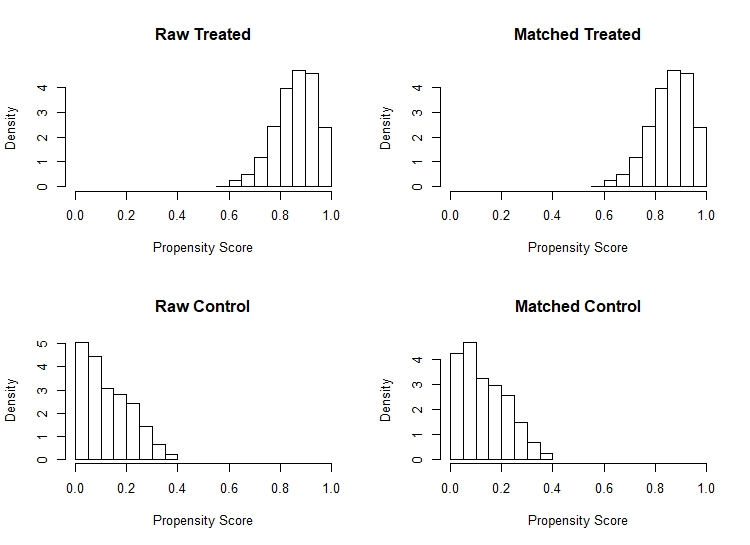
\includegraphics[width=\linewidth]{Figures/local_rf_nonpara_hist.jpeg}
        \caption{Random Forest after FS}\label{fig:histogram6}
    \endminipage\hfill
    \minipage{0.5\textwidth}%
        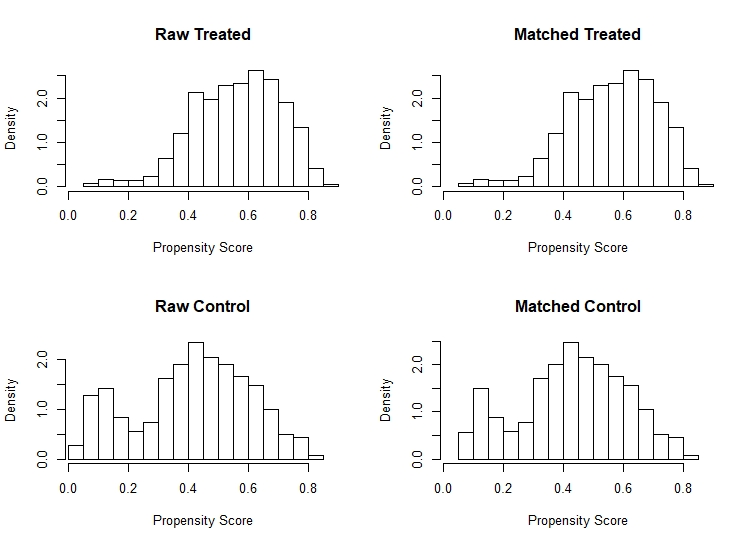
\includegraphics[width=\linewidth]{Figures/local_xgb_hist.jpeg}
        \caption{XGBoost after FS}\label{fig:histogram7}
    \endminipage
\end{figure}

\par
On the contrary, traditional Logit model, Linear SVM model and XGBoost model produce distributions which are quite similar to each other. The resulting distributions are shown in figure one, two, five, and seven, respectively. Not like Raidal SVM and Random Forest models, they generate distributions which shapes appear to be more bell-shaped as normal distribution. However, the distributions from Linear SVM and XGBoost models are slightly skewed. For instance of XGBoost (figure five and seven), the distributions of the control groups have a small spike at the left-hand side, and are slightly right skewed. The distributions of the treated groups are slightly left skewed, having more observations with a  propensity score around 0.6. 
\par
Similar patterns are also shown in figure one and two, and the two figures considerably resemble each other. This is due to the fact the two models behave in a similar manner (Koller et al, 2007, p.356).\cite{koller2007introduction} In chapter 9.5 of the book, \emph{Introduction to Statistical Learning} (Koller et al., 2007)\cite{koller2007introduction}, it is written loss functions of logistic regression and Linear SVM, or Support Vector Classifier, share similarities. Morover, Linear SVM tends to perform better than Logit if classes are well divided, like in this case. If not, logistic regression is preferred.
\par
To summarize, not all machine learning methods do not satisfy common support assumption, especially in a sense that a machine learning method does not generate an overlapping region in propensity score distributions between the treated and the non-treated. Specifically, Random Forest method produces biased propensity scores depending on an observation belongs to a control group or a treatment group. However, some models, such as Linear SVM, XGBoost, and Logit model result in rather similar distributions between the treated and the control.
\\\\
$\bullet$ \textbf{Numerical Diagnostics}\\
I use standardized difference in means of propensity scores\footnote{It will be often referred as "the standardized difference" or "standardized difference of means"} and the ratio of the variances of the propensity score\footnote{The term, "the variance ratio" will be interchangably used} in the two groups, the treated and the control, as the numerical diagnostics to check the quality of matching. The measure is introduced in Rubin (2001).\cite{rubin2001using} Moreover, the paper argues the standardized difference should be below 0.5, and the variance ratio should be close to one or at least should be between 0.5 and 2. 
\par
The equations to calculate the standardized difference and the variance ratio is shown below.
\begin{align*}
    \text{Standardized Difference of Means} &= \frac{\mu_{T} - \mu_{C}}{\sigma_{T}}\\
    \text{Variance Ratio} &= \frac{\sigma^{2}_{T}}{\sigma^{2}_{C}}
\end{align*}
$\mu_{T}$ denotes the mean of propensity scores of the treated group; $\mu_{C}$ is the mean of propensity scores of the control group; $\sigma_{T}$ is the standard deviation of propensity scores of the treatment group; and $\sigma_{C}$ is the standard deviation of propensity scores of the control group.
\par
Table 4 shows the two numerical diagnostics and some additional information by each statistical model. The standardized difference is shown in the third column, and the fourth column shows the variance ratio. The first two columns present the means of propensity scores in both groups: the treated and the control. Lastly, the fifth column tells us how much percentage reduction has occurred in the standardized difference after matching.
\begin{table}[t!]
	\centering
	\caption{Numerical Diagnostics of Matching Quality (Local)}
	\begin{threeparttable}
	{\def\arraystretch{0.7}\setlength{\tabcolsep}{3pt}
	\begin{tabular}{*6c} 
		\toprule {} & \multicolumn{4}{c}{Propensity Score}\\
		\multirow{2}{*}{Method} & \multirow{2}{*}{Mean} & \multirow{2}{*}{Mean} & \multirow{2}{*}{Std. Diff} & \multirow{2}{*}{Variance} & \multirow{2}{*}{Reduction}\\
		\multirow{2}{*}{} & \multirow{2}{*}{Treated} & \multirow{2}{*}{Control} & \multirow{2}{*}{of Means} & \multirow{2}{*}{Ratio} & \multirow{2}{*}{(\%)}\\\\
		\midrule
		\multicolumn{1}{l}{Logit} & \multicolumn{1}{r}{0.523} & \multicolumn{1}{r}{0.463} & \multicolumn{1}{r}{0.528} & \multicolumn{1}{r}{0.754} & \multicolumn{1}{r}{15.447}\\
		\multicolumn{1}{l}{Linear SVM} & \multicolumn{1}{r}{0.521} & \multicolumn{1}{r}{0.462} & \multicolumn{1}{r}{0.530} & \multicolumn{1}{r}{0.779} & \multicolumn{1}{r}{12.959}\\
		\multicolumn{1}{l}{Radial SVM} & \multicolumn{1}{r}{0.555} & \multicolumn{1}{r}{0.437} & \multicolumn{1}{r}{0.919} & \multicolumn{1}{r}{0.797} & \multicolumn{1}{r}{7.263}\\
		\multicolumn{1}{l}{Random Forest} & \multicolumn{1}{r}{0.832} & \multicolumn{1}{r}{0.165} & \multicolumn{1}{r}{9.107} & \multicolumn{1}{r}{0.710} & \multicolumn{1}{r}{1.238}\\
		\multicolumn{1}{l}{XGBoost} & \multicolumn{1}{r}{0.568} & \multicolumn{1}{r}{0.429} & \multicolumn{1}{r}{0.958} & \multicolumn{1}{r}{0.689} & \multicolumn{1}{r}{12.345}\\
		\multicolumn{1}{l}{\multirow{2}{*}{Random Forest}} & \multicolumn{1}{r}{\multirow{2}{*}{0.865}} & \multicolumn{1}{r}{\multirow{2}{*}{0.133}} & \multicolumn{1}{r}{\multirow{2}{*}{9.438}} & \multicolumn{1}{r}{\multirow{2}{*}{0.732}} & \multicolumn{1}{r}{\multirow{2}{*}{0.937}}\\
		\multicolumn{1}{l}{\multirow{2}{*}{after feature selection}} & \multicolumn{1}{r}{\multirow{2}{*}{}}  & \multicolumn{1}{r}{\multirow{2}{*}{}} & \multicolumn{1}{r}{\multirow{2}{*}{}} & \multicolumn{1}{r}{\multirow{2}{*}{}} & \multicolumn{1}{r}{\multirow{2}{*}{}}\\
		\multicolumn{1}{l}{\multirow{2}{*}{XGBoost}} & \multicolumn{1}{r}{\multirow{2}{*}{0.668}} & \multicolumn{1}{r}{\multirow{2}{*}{0.324}} & \multicolumn{1}{r}{\multirow{2}{*}{2.037}}  & \multicolumn{1}{r}{\multirow{2}{*}{0.568}}& \multicolumn{1}{r}{\multirow{2}{*}{4.584}}\\
		\multicolumn{1}{l}{\multirow{2}{*}{after feature selection}} & \multicolumn{1}{r}{\multirow{2}{*}{}} & \multicolumn{1}{r}{\multirow{2}{*}{}} & \multicolumn{1}{r}{\multirow{2}{*}{}} &  \multicolumn{1}{r}{\multirow{2}{*}{}} & \multicolumn{1}{r}{\multirow{2}{*}{}}\\\\
		\bottomrule
	\end{tabular}
	}
	\begin{tablenotes}[para,flushleft]
	    \linespread{1}\footnotesize
	    Note: The standardized difference is shown in the third column, and the fourth column shows the variance ratio. The first two columns present the means of propensity scores in both groups: the treated and the non-treated. The fifth column tells us how much percentage reduction has occurred in the standardized difference after matching.
	\end{tablenotes}
	\end{threeparttable}
	\label{table:4}
\end{table}
\par
Unfortunately, no statistical model produces the standardized difference of means which is lower than 0.5.  Two Random Forest models result in the highest values of the standardized difference. Without feature selection process, the model produces a value of 9.107 and 9.438, after feature selection. It is predictable results as the distribution of the propensity scores are extremely skewed to either end in each group. Hence, the mean of propensity scores of the treated group is considerably high. Both of the mean values exceed 0.8. The mean values of the control groups, however, are substantially low, and are lower than 0.2 Another variation of Tree methods, XGBoost also generates relatively high value in standardized difference. When the model is trained with five basic matching variables, it results in 0.958 standardized difference. With more matching variables chosen, after feature selection, the trained model produces standardized difference with a value of 2.037. 
\par
The two versions of SVM model and the Logit model also have standardized difference values which are larger than 0.5. The Linear SVM, however, has a lower value than the Radial SVM model and the Logit model by approximately 0.4. It is due to the fact that Radial SVM has higher mean difference between the treated. One should notice that the Logit model has the closest value to the threshold value of standardized difference, 0.5, not the other machine learning models. Moreover, the traditional logistic regression has the highest percentage reduction in standardized difference (15.4\%). It could be interpreted as the Logit model has resulted in much better covariate balance than other statistical models. The second largest value is produced by a close relative of the Logit model, the Linear SVM.
\par
In terms of variance ratio, Radial SVM has the closed value to one (0.797), and it is followed by the values of the Linear SVM and the Logit model: 0.779 and 0.754, respectively. Also, two Random Forest models have variance ratio values which are relatively close to one as the values are all more than 0.7. The Logit model and the Linear SVM model enjoys close-to-one variance ratio values as they both have rather similar propensity scores distribution in the treated and the control. In case of Radil SVM model and Random Forest models, they have variance ratio values close to one because these models have skewed distributions. The treated groups of the three models have a left skewed distribution, and the non-treatedhave right skewed distribution. As a result, both groups have relatively low standard deviation. Interestingly, two XGBoost models resulted in the lowest variance ratio: 0.689 and 0.568. Such low values are produced because the distribution of propensity scores of the control group has a small spike at the left end in both models, which is a clear difference from the distribution of the treated. Subsequently, the variance of the control group is relatively larger than the variance of the treated group, resulting in a low value of the variance ratio.
\\\\
$\bullet$ \textbf{Summary}\\
Combining the results I have shown in this subsection, implementing machine learning methods to calculate propensity scores, at least, do not lead to better matching quality, and even could be said the traditional logistic regression produces the best matching quality in the setting of this study. All the machine learning models generate larger values of the standardized difference which are all above the threshold value, 0.5, and the Logit model results in the standardized difference of means with a value closest to 0.5 (0.528). In addition, the variance ratio value of the Logit model is close to one, and has the highest percentage reduction rate: 15.447\%.

%============================================================================================
\subsubsection{Global control group}
\begin{figure}[!t]
    \minipage{0.5\textwidth}
  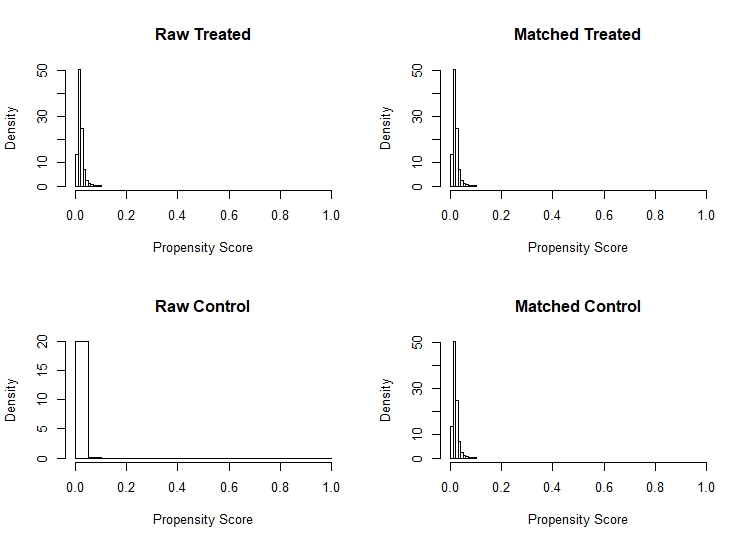
\includegraphics[width=\linewidth]{Figures/global_logit_hist.jpeg}
  \caption{Logit}\label{fig:histogram_global1}
\endminipage
\minipage{0.5\textwidth}
  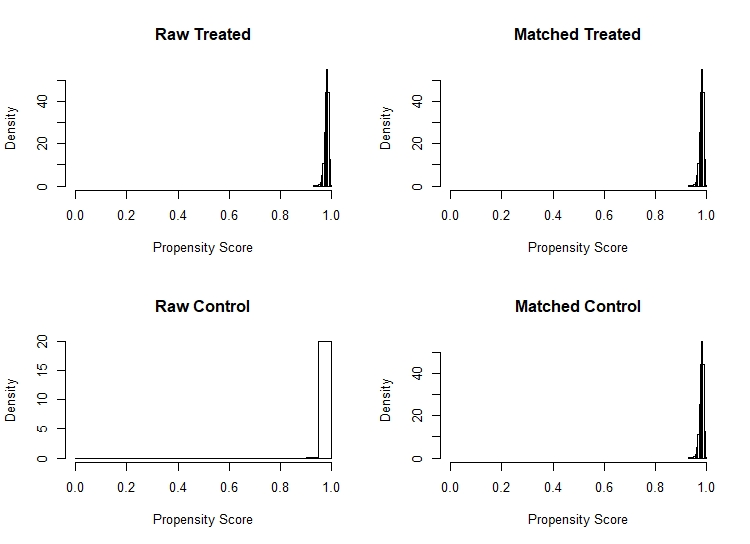
\includegraphics[width=\linewidth]{Figures/global_svm_hist.jpeg}
  \caption{Linear SVM}\label{fig:histogram_global2}
\endminipage\hfill
\minipage{0.5\textwidth}%
  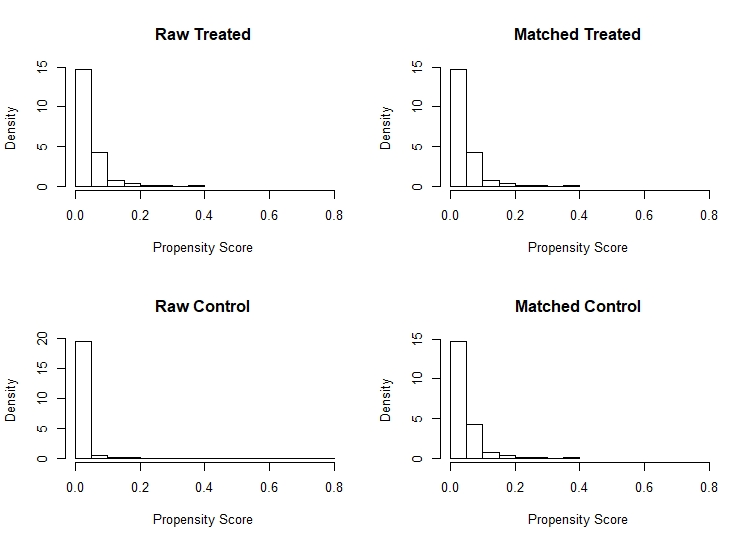
\includegraphics[width=\linewidth]{Figures/global_xgb_hist.jpeg}
  \caption{XGBoost}\label{fig:histogram3}
\endminipage
\minipage{0.5\textwidth}
  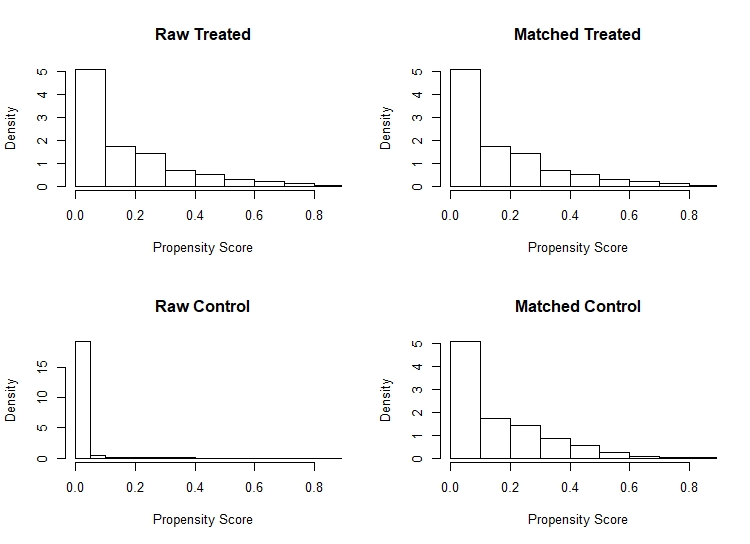
\includegraphics[width=\linewidth]{Figures/global_xgb_non_para_hist.jpeg}
  \caption{XGBoost after FS}\label{fig:histogram_global4}
\endminipage
\end{figure}

From the results using local control group, among the two SVM models, Linear SVM has performed better than Radial SVM, and the performance of XGBoost model is better than other Random Forest models. Thus, only Logit, Linear SVM, XGBoost, and XGBoost after feature selection(FS) are considered in this subsection. Radial SVM model and Random Forest models are excluded from the analysis as the models require substantial computation time: several days. However, Radial SVM and Random Forest models also produce similar results, which would be shown shortly after, with slightly different data cleaning process.\footnote{Non-parametric data had different observation from the original data and central imputation process was conducted on the whole dataset, not by each firm.} 


$\bullet$ \textbf{Region of Common Support}\\
The propensity score histogram now looks clearly dissimilar from the histograms produced with local control group. All of the models are predicting extreme results: most of the observations will either be treated or not treated. Linear SVM model is the only model which expects most of the majority of observations to be treated, having propensity scores highly concentrated over 0.9. However, the other three models predict most observations not to be treated, and the estimated propensity scores by the tree models are mostly lower than 0.2. However, it does seem the estimated propensity score distributions of the treated and the non-treatedoverlap each other well.
\\\\
$\bullet$ \textbf{Numerical Diagnostics}\\
\begin{table}[t!]
	\centering
	\caption{Numerical Diagnostics of Matching Quality (Global)}
	\begin{threeparttable}
	{\def\arraystretch{0.7}\setlength{\tabcolsep}{3pt}
	\begin{tabular}{*6c} 
		\toprule {} & \multicolumn{4}{c}{Propensity Score}\\
		\multirow{2}{*}{Method} & \multirow{2}{*}{Mean} & \multirow{2}{*}{Mean} & \multirow{2}{*}{Std. Diff} & \multirow{2}{*}{Variance} & \multirow{2}{*}{Reduction}\\
		\multirow{2}{*}{} & \multirow{2}{*}{Treated} & \multirow{2}{*}{Control} & \multirow{2}{*}{of Means} & \multirow{2}{*}{Ratio} & \multirow{2}{*}{(\%)}\\\\
		\midrule
		\multicolumn{1}{l}{Logit} & \multicolumn{1}{r}{0.019} & \multicolumn{1}{r}{0.019} & \multicolumn{1}{r}{0.000} & \multicolumn{1}{r}{1.000} & \multicolumn{1}{r}{99.996}\\
		\multicolumn{1}{l}{Linear SVM} & \multicolumn{1}{r}{0.980} & \multicolumn{1}{r}{0.980} & \multicolumn{1}{r}{0.000} & \multicolumn{1}{r}{1.001} & \multicolumn{1}{r}{99.988}\\
		\multicolumn{1}{l}{XGBoost} & \multicolumn{1}{r}{0.041} & \multicolumn{1}{r}{0.041} & \multicolumn{1}{r}{0.000} & \multicolumn{1}{r}{1.001} & \multicolumn{1}{r}{99.991}\\
		\multicolumn{1}{l}{\multirow{2}{*}{XGBoost}} & \multicolumn{1}{r}{\multirow{2}{*}{0.163}} & \multicolumn{1}{r}{\multirow{2}{*}{0.156}} & \multicolumn{1}{r}{\multirow{2}{*}{0.039}}  & \multicolumn{1}{r}{\multirow{2}{*}{1.207}} & \multicolumn{1}{r}{\multirow{2}{*}{95.476}}\\
		\multicolumn{1}{l}{\multirow{2}{*}{after feature selection}} & \multicolumn{1}{r}{\multirow{2}{*}{}} & \multicolumn{1}{r}{\multirow{2}{*}{}} & \multicolumn{1}{r}{\multirow{2}{*}{}} &  \multicolumn{1}{r}{\multirow{2}{*}{}} & \multicolumn{1}{r}{\multirow{2}{*}{}}\\\\
		\bottomrule
	\end{tabular}
	}
	\begin{tablenotes}[para,flushleft]
	    \linespread{1}\footnotesize
	    Note: The standardized difference is shown in the third column, and the fourth column shows the variance ratio. The first two columns present the means of propensity scores in both groups: the treated and the non-treated. The fifth column tells us how much percentage reduction has occurred in the standardized difference after matching.
	\end{tablenotes}
	\end{threeparttable}
	\label{table:5}
\end{table}

All statistical models have resulted in which could be claimed as perfect matching. The standardized difference in means of propensity scores are all lower than 0.1, and every value of the variance ratios is close to 1. The reduction rate of the standardized difference after matching is also very high but it conveys little meaning because the treatment share is only 1.5\% in this case. Among the four models, XGBoost after feature selection performs the worst as its deviation from zero and one in two covariate balance values is larger than any other models. In fact, the traditional logistic regression is again one of the models producing the best matching quality. 
%============================================================================================
%============================================================================================
\subsection{Pooled OLS}
The result of analyzing the effect of minimum wage introduction on capital-labor ratio of firms is shown in this subsection. A simple pooled OLS regression is conducted on generated matched data by multiple statistical models which I have mentioned in previous sections. The regression equation is identical as in Gathmann et al.(2018)\cite{Gathmann2018}, and is as the following:
\begin{align}
    Y_{it} \;=\; \beta_{0t} \;+\; \beta_{1t}*T \;+\; \gamma_{i} \;+\; \epsilon_{it}.
\end{align}
$i$ denotes an individual firm, and $t$ is an year variable ranging from 2007 to 2013. $Y_{it}$ is the capital-labor ratio of a firm $i$ at time $t$. $\gamma_{i}$ is firm fixed effect, and $\epsilon_{it}$ is the error term. $T$ is a dummy variable which has a value of one if a firm is Nursing and Caring sector. Hence, $\beta_{1t}$ measures the effect of minimum wage introduction on a firm's capital-labor ratio, and $\beta_{0t}$ is time-fixed effect.
\par
Note that minimum wage was introduced in 2010 for workers in Nursing and Caring sector. Therefore, $\beta_{1t}$ in equation (14) will measure systematic difference in capital-labor ratio between firms in Nursing and Caring sector and the others if $t<2010$. For $t\geq2010$, the coefficient will measure the impact of minimum wage introduction on capital-labor ratio, which is our variable of interest.
\subsubsection{Local control group}
\par
The values of $\beta_{1t}$ are shown in Table 5 and Table 6. Note that these results are driven by using local control group. The header of each column represents the statistical model implemented to calculate propensity scores for matching, and the matched data generated from the according matching procedure is used for the pooled OLS.

\begin{table}[!t]
	\centering
	\caption{Pooled OLS Result part 1 (Local)}
	\begin{threeparttable}
	\def\arraystretch{0.7}
	\begin{tabular}{*7c}
		\toprule 
		{Model }  & \multicolumn{2}{c}{Logit} & \multicolumn{2}{c}{Linear SVM} & \multicolumn{2}{c}{Radial SVM}\\
		{Year} & \multicolumn{2}{c}{Coefficient} & \multicolumn{2}{c}{Coefficient} & \multicolumn{2}{c}{Coefficient}\\
		\midrule
		\multicolumn{1}{l}{2007} & \multicolumn{2}{c}{-0.0148} & \multicolumn{2}{c}{-0.0154} & \multicolumn{2}{c}{0.0027}\\
		\multicolumn{1}{l}{} & \multicolumn{2}{c}{(0.0336)} & \multicolumn{2}{c}{(0.0337)} & \multicolumn{2}{c}{(0.0337)}\\
		
		\multicolumn{1}{l}{2008} & \multicolumn{2}{c}{0.0194} & \multicolumn{2}{c}{0.0183} & \multicolumn{2}{c}{0.0267}\\
		\multicolumn{1}{l}{} & \multicolumn{2}{c}{(0.0240)} & \multicolumn{2}{c}{(0.0240)} & \multicolumn{2}{c}{(0.0248)}\\
		
		\multicolumn{1}{l}{2009} & \multicolumn{2}{c}{0.0346*} & \multicolumn{2}{c}{0.0340*} & \multicolumn{2}{c}{0.0398**}\\
		\multicolumn{1}{l}{} & \multicolumn{2}{c}{(0.0195)} & \multicolumn{2}{c}{(0.0194)} & \multicolumn{2}{c}{(0.0196)}\\
		
		\multicolumn{1}{l}{2010} & \multicolumn{2}{c}{0.0180} & \multicolumn{2}{c}{0.0175} & \multicolumn{2}{c}{0.0116}\\
		\multicolumn{1}{l}{} & \multicolumn{2}{c}{(0.0183)} & \multicolumn{2}{c}{(0.0183)} & \multicolumn{2}{c}{(0.0182)}\\
		
		\multicolumn{1}{l}{2011} & \multicolumn{2}{c}{-0.0077} & \multicolumn{2}{c}{-0.0064} & \multicolumn{2}{c}{-0.0143}\\
		\multicolumn{1}{l}{} & \multicolumn{2}{c}{(0.0189)} & \multicolumn{2}{c}{(0.0188)} & \multicolumn{2}{c}{(0.0190)}\\
		
		\multicolumn{1}{l}{2012} & \multicolumn{2}{c}{-0.0241} & \multicolumn{2}{c}{-0.0214} & \multicolumn{2}{c}{-0.0298}\\
		\multicolumn{1}{l}{} & \multicolumn{2}{c}{(0.0216)} & \multicolumn{2}{c}{(0.0217)} & \multicolumn{2}{c}{(0.0219)}\\
		
		\multicolumn{1}{l}{2013} & \multicolumn{2}{c}{-0.0255} & \multicolumn{2}{c}{-0.0266} & \multicolumn{2}{c}{-0.0366}\\
		\multicolumn{1}{l}{} & \multicolumn{2}{c}{(0.0267)} & \multicolumn{2}{c}{(0.0269)} & \multicolumn{2}{c}{(0.0271)}\\
		\bottomrule
	\end{tabular}
	\begin{tablenotes}[para,flushleft]
	    \linespread{1}\footnotesize
	    Note: Each column shows coefficient of the industry indicator. The outcome variable is the capital-labor ratio. The values of coefficients are produced by conducting a pooled OLS regression with a matched dataset resulted by using according statistical model to calculate propensity scores. Standard errors are in parentheses. Statistical significance is indicated by the number of asterisk symbols. *: $p<0.10$, **: $p<0.05$, ***: $p<0.01$.
	\end{tablenotes}
	\end{threeparttable}
	\label{table:6}
\end{table}

\par
Besides, Radial SVM model, all the models share identical pattern and have similar coefficient size in each year. For instance, the sign of the coefficient is negative in year 2007 and year from 2011 to 2013, and the coefficient has a positive sign in year 2008, 2009, and 2010. Radial SVM model also has much similar pattern but the sign of the coefficient in 2007 is positive. In addition, the coefficient value in year 2009 is statistically significant at least at 10\% level. Only when Radial SVM model is used to calculate propensity scores, the coefficient of interest has a p-value less than 0.05. Moreover, the values of the coefficient in year 2009 range approximately from 0.034 to 0.040. This could be interpreted as firms in Nursing and Caring sector have systematically higher capital-labor ratio than other firms which have not been affected by minimum wage introduction by approximately 3.4\% points in year 2009.

\begin{table}[!t]
	\centering
	\caption{Pooled OLS Result part 2 (Local)}
	\begin{threeparttable}
	\def\arraystretch{0.7}
	\begin{tabular}{*9c}
		\toprule 
		\multirow{2}{*}{Model}  & \multicolumn{2}{c}{\multirow{2}{*}{Random Forest}} & \multicolumn{2}{c}{\multirow{2}{*}{XGBoost}} & \multicolumn{2}{c}{Random Forest} & \multicolumn{2}{c}{XGBoost}\\
		{} & \multicolumn{2}{c}{} & \multicolumn{2}{c}{} & \multicolumn{2}{c}{after FS} & \multicolumn{2}{c}{after FS}\\
		{Year} & \multicolumn{2}{c}{Coefficient} & \multicolumn{2}{c}{Coefficient} & \multicolumn{2}{c}{Coefficient} & \multicolumn{2}{c}{Coefficient}\\
		\midrule
		\multicolumn{1}{l}{2007} & \multicolumn{2}{c}{-0.0089} & \multicolumn{2}{c}{-0.0107} & \multicolumn{2}{c}{-0.0093}& \multicolumn{2}{c}{-0.0105}\\
		\multicolumn{1}{l}{} & \multicolumn{2}{c}{(0.0338)} & \multicolumn{2}{c}{(0.0338)} & \multicolumn{2}{c}{(0.0340)}& \multicolumn{2}{c}{(0.0338)}\\
		
		\multicolumn{1}{l}{2008} & \multicolumn{2}{c}{0.0198} & \multicolumn{2}{c}{0.0274} & \multicolumn{2}{c}{0.0198}& \multicolumn{2}{c}{0.0193}\\
		\multicolumn{1}{l}{} & \multicolumn{2}{c}{(0.0248)} & \multicolumn{2}{c}{(0.0245)} & \multicolumn{2}{c}{(0.0249)}& \multicolumn{2}{c}{(0.0248)}\\
		
		\multicolumn{1}{l}{2009} & \multicolumn{2}{c}{0.0339*} & \multicolumn{2}{c}{0.0344*} & \multicolumn{2}{c}{0.0362*}& \multicolumn{2}{c}{0.0346*}\\
		\multicolumn{1}{l}{} & \multicolumn{2}{c}{(0.0196)} & \multicolumn{2}{c}{(0.0196)} & \multicolumn{2}{c}{(0.0197)}& \multicolumn{2}{c}{(0.0196)}\\
		
		\multicolumn{1}{l}{2010} & \multicolumn{2}{c}{0.0159} & \multicolumn{2}{c}{0.0165} & \multicolumn{2}{c}{0.0179} & \multicolumn{2}{c}{0.0171}\\
		\multicolumn{1}{l}{} & \multicolumn{2}{c}{(0.0185)} & \multicolumn{2}{c}{(0.0185)} & \multicolumn{2}{c}{(0.0185)}& \multicolumn{2}{c}{(0.0185)}\\
		
		\multicolumn{1}{l}{2011} & \multicolumn{2}{c}{-0.0082} & \multicolumn{2}{c}{-0.0106} & \multicolumn{2}{c}{-0.0095} & \multicolumn{2}{c}{-0.0087}\\
		\multicolumn{1}{l}{} & \multicolumn{2}{c}{(0.0190)} & \multicolumn{2}{c}{(0.0190)} & \multicolumn{2}{c}{(0.0191)} & \multicolumn{2}{c}{(0.0190)}\\
		
		\multicolumn{1}{l}{2012} & \multicolumn{2}{c}{-0.0243} & \multicolumn{2}{c}{-0.0262} & \multicolumn{2}{c}{-0.0274} & \multicolumn{2}{c}{-0.0237}\\
		\multicolumn{1}{l}{} & \multicolumn{2}{c}{(0.0219)} & \multicolumn{2}{c}{(0.0220)} & \multicolumn{2}{c}{(0.0219)}& \multicolumn{2}{c}{(0.0220)}\\
		
		\multicolumn{1}{l}{2013} & \multicolumn{2}{c}{-0.0281} & \multicolumn{2}{c}{-0.0307} & \multicolumn{2}{c}{-0.0277} & \multicolumn{2}{c}{-0.0280}\\
		\multicolumn{1}{l}{} & \multicolumn{2}{c}{(0.0271)} & \multicolumn{2}{c}{(0.0271)} & \multicolumn{2}{c}{(0.0271)}& \multicolumn{2}{c}{(0.0271)}\\
		\bottomrule
	\end{tabular}
	\begin{tablenotes}[para,flushleft]
	    \linespread{1}\footnotesize
	     Note: Each column shows coefficient of the industry indicator. The outcome variable is the capital-labor ratio. The values of coefficients are produced by conducting a pooled OLS regression with a matched dataset resulted by using according statistical model to calculate propensity scores. Standard errors are in parentheses. Statistical significance is indicated by the number of asterisk symbols. *: $p<0.10$, **: $p<0.05$, ***: $p<0.01$.
	\end{tablenotes}
	\end{threeparttable}
	\label{table:7}
\end{table}

\par
In simple way of thinking, the coefficient values of year 2009 could be seen as an attempt of the firms in Nursing and Caring industry to minimize the impact of minimum wage introduction in year 2010. Indeed, the firms in Nursing and Caring sector have systematically higher capital, or fixed assets to be precise, in year 2009 compared to other firms which are not affected by minimum wage. The significance level is also at 10\% level. If the outcome variable of pooled OLS is replaced by the log value of total number of employees, the resulting coefficient, $\beta_{1t}$, has a negative sign but not statistically significant.

%============================================================================================
\subsection{Global control group}
\begin{table}[!t]
	\centering
	\caption{Pooled OLS Result (Global)}
	\begin{threeparttable}
	\def\arraystretch{0.7}
	\begin{tabular}{*9c}
		\toprule 
		\multirow{2}{*}{Model}  & \multicolumn{2}{c}{\multirow{2}{*}{Logit}} & \multicolumn{2}{c}{\multirow{2}{*}{Linear SVM}} & \multicolumn{2}{c}{XGBoost} & \multicolumn{2}{c}{XGBoost}\\
		{} & \multicolumn{2}{c}{} & \multicolumn{2}{c}{} & \multicolumn{2}{c}{} & \multicolumn{2}{c}{after FS}\\
		{Year} & \multicolumn{2}{c}{Coefficient} & \multicolumn{2}{c}{Coefficient} & \multicolumn{2}{c}{Coefficient} & \multicolumn{2}{c}{Coefficient}\\
		\midrule
		\multicolumn{1}{l}{2007} & \multicolumn{2}{c}{0.0273} & \multicolumn{2}{c}{0.0734**} & \multicolumn{2}{c}{0.1399***}& \multicolumn{2}{c}{0.0099}\\
		\multicolumn{1}{l}{} & \multicolumn{2}{c}{(0.0358)} & \multicolumn{2}{c}{(0.0361)} & \multicolumn{2}{c}{(0.0374)}& \multicolumn{2}{c}{(0.0347)}\\
		
		\multicolumn{1}{l}{2008} & \multicolumn{2}{c}{-0.0123} & \multicolumn{2}{c}{0.0307} & \multicolumn{2}{c}{0.1444***}& \multicolumn{2}{c}{0.1044***}\\
		\multicolumn{1}{l}{} & \multicolumn{2}{c}{(0.0247)} & \multicolumn{2}{c}{(0.0252)} & \multicolumn{2}{c}{(0.0265)}& \multicolumn{2}{c}{(0.0247)}\\
		
		\multicolumn{1}{l}{2009} & \multicolumn{2}{c}{0.0268} & \multicolumn{2}{c}{0.0479**} & \multicolumn{2}{c}{0.0707***}& \multicolumn{2}{c}{0.1130***}\\
		\multicolumn{1}{l}{} & \multicolumn{2}{c}{(0.0202)} & \multicolumn{2}{c}{(0.0211)} & \multicolumn{2}{c}{(0.0210)}& \multicolumn{2}{c}{(0.0209)}\\
		
		\multicolumn{1}{l}{2010} & \multicolumn{2}{c}{0.0263} & \multicolumn{2}{c}{0.0136} & \multicolumn{2}{c}{-0.0103} & \multicolumn{2}{c}{0.0315*}\\
		\multicolumn{1}{l}{} & \multicolumn{2}{c}{(0.0190)} & \multicolumn{2}{c}{(0.0196)} & \multicolumn{2}{c}{(0.0191)}& \multicolumn{2}{c}{(0.0181)}\\
		
		\multicolumn{1}{l}{2011} & \multicolumn{2}{c}{0.0087} & \multicolumn{2}{c}{-0.0446**} & \multicolumn{2}{c}{-0.0876**} & \multicolumn{2}{c}{-0.0537***}\\
		\multicolumn{1}{l}{} & \multicolumn{2}{c}{(0.0195)} & \multicolumn{2}{c}{(0.0207)} & \multicolumn{2}{c}{(0.0203)} & \multicolumn{2}{c}{(0.0199)}\\
		
		\multicolumn{1}{l}{2012} & \multicolumn{2}{c}{-0.0244} & \multicolumn{2}{c}{-0.0622***} & \multicolumn{2}{c}{-0.1151***} & \multicolumn{2}{c}{-0.0995***}\\
		\multicolumn{1}{l}{} & \multicolumn{2}{c}{(0.0222)} & \multicolumn{2}{c}{(0.0230)} & \multicolumn{2}{c}{(0.0231)}& \multicolumn{2}{c}{(0.0221)}\\
		
		\multicolumn{1}{l}{2013} & \multicolumn{2}{c}{-0.0524} & \multicolumn{2}{c}{-0.0587**} & \multicolumn{2}{c}{-0.1419***} & \multicolumn{2}{c}{-0.1056***}\\
		\multicolumn{1}{l}{} & \multicolumn{2}{c}{(0.0273)} & \multicolumn{2}{c}{(0.0273)} & \multicolumn{2}{c}{(0.0283)}& \multicolumn{2}{c}{(0.0282)}\\
		\bottomrule
	\end{tabular}
	\begin{tablenotes}[para,flushleft]
	    \linespread{1}\footnotesize
%============================================================================================
	     Note: Each column shows coefficient of the industry indicator. The outcome variable is the capital-labor ratio. The values of coefficients are produced by conducting a pooled OLS regression with a matched dataset resulted by using according statistical model to calculate propensity scores. Standard errors are in parentheses. Statistical significance is indicated by the number of asterisk symbols. *: $p<0.10$, **: $p<0.05$, ***: $p<0.01$.
	\end{tablenotes}
	\end{threeparttable}
	\label{table:8}
\end{table}

The pooled OLS results by having the global control group are shown in Table 8. The result of traditional model is absolutely different from other three machine learning models. The coefficient of the industry indicator is statistically insignificant in all years. However, for the machine learning models, industry indicator has, at least, strong correlation in years except 2008 and 2010. After, 2010 all the machine learning methods show strong negative correlation exists between the industry indicator and the capital-labor ratio. In year 2007 and 2010, machine learning methods believe positive statistical relationship exists between the industry indicator and the capital-labor ratio. As the results are not consistent in every model, it is difficult to infer based on these results.
%============================================================================================
%============================================================================================
%============================================================================================

\section{Discussion}


\subsection{Possible reasons why machine learning underperforms}
The difference between the objective of calculating propensity scores in matching and the objective of machine learning might drive Logit model to overperform other four machine learning models. In matching, propensity scores are calculated to achieve covariate balance, and choose the most similar observations to treated observations, which could be used as the potential control group. However, the sole target of machine learning is to obtain highest accuracy rate, no matter what it takes. Hence, extreme cases as Random Forest models in section 5.2.1 might occur, resulting in no overlap in propensity score distributions between the treated group and the control group but having a high prediction rate.

\subsection{Shortcomings of the paper}
Several shortcomings exist in this study. Firstly, the variables included in global non-parametric data are different from the ones in local non-parametric data, and imputation process is also different, not allowing us to have clear comparison between results with different control data. In addition, Radial SVM and Random Forest models are not implemented on global dataset, which could have given us much more clear insight from this study. 
\par
Additional Robust check could have been conducted by varying the treatment share in the dataset. In this paper, only two extreme cases are considered: when the treatment share is roughly 45\% and when it is around 1\%. It would be interesting to test whether the treatment share have large impact on resulting matching quality from statistical models. Hence, future studies should be done to overcome these shortcomings in this study.
%============================================================================================
%============================================================================================

\section{Conclusion}

I have reviewed four different machine learning methods whether applying the methods to calculate propensity scores would produce better matching quality than when traditional Logit model is implemented. The setting of this paper is of minimum wage introduction in west Germany in a certain sector, and partly focuses on to measure the impact of minimum wage introduction (ATT). 
\par
Propensity scores are calculated in various ways by changing the matching variables and changing the size of the control group. Then, matching quality is quantified using two main numerical diagnostics: the standardized difference in means of propensity scores and the variance ratio of propensity scores between the treated and the non-treated.
\par
When the global control group is used, the two diagnostics suggest machine learning methods, at least in this paper setting, do not overperform than the Logit model, and, even, some of the models have worse matching quality than the logistic regression. The results of pooled OLS after matching are unclear. Estimated coefficients of being treated have no statistical significance in every year when the Logit model is implemented. However, if the Linear SVM, and two XGBoost models are used to calculate propensity scores, the estimated coefficients mostly are statistically significant besides few years. In addition, the coefficients suggest a positive relationship exists between the industry indicator and the capital-labor ratio of a firm before 2010 but a negative one after 2010.
\par
However, inference is quite clear in the local control group case. As in the results of global control group, Logit models does not underperform than other machine learning models but rather performs better than some of the models. Moreover, the results of pooled OLS from different statistical methods are consistent. All the treatment variables have statistical significance at 10\% level in year 2009. The magnitude of the variable is also stable, and it is approximately, 0.034. This would mean the firms in Nursing and Caring sector have systematically higher capital-labor ratio than other non-treated firms in year 2009. However, the interpretation and the mechanism behind this result are unclear.

\par
To summarize, this study suggests that no clear evidence has been found or exists supporting that implementing machine learning methods into matching improves matching quality. On the contrary, it is advisable to use traditional Logit model for propensity score matching if we consider the complexity of building a machine learning model for calculating propensity scores, based on the results of this study. Future studies should be done on different setting, with different machine learning methods to acquire a clear answer to the research question of this paper.
%============================================================================================
%============================================================================================
%============================================================================================
\newpage
\bibliographystyle{acm}
\bibliography{main}
%============================================================================================
%============================================================================================
%============================================================================================
\newpage
\section{Appendix}
\subsection{Technical information}
R version of 3.6.1 and RStudio with a version of 1.2.1335 was used for my analysis. Furthermore, I list all the packages which are necessary for this study.

\begin{table}[h!]
 \renewcommand\thetable{A.1}
	\centering
	\caption{R packages}
	\begin{threeparttable}
	\def\arraystretch{1}
	\begin{tabular}{*3c}
	\hline
    \multicolumn{1}{r}{ caret} &    \multicolumn{1}{r}{ caTools} &    \multicolumn{1}{r}{ haven}\\
    \multicolumn{1}{r}{ dplyr} &    \multicolumn{1}{r}{ MatchIt} &    \multicolumn{1}{r}{ gridExtra}\\
    \multicolumn{1}{r}{ e1071} &    \multicolumn{1}{r}{ stats} &    \multicolumn{1}{r}{ ggplot2}\\
    \multicolumn{1}{r}{ randomForest} &    \multicolumn{1}{r}{ stringr} &    \multicolumn{1}{r}{ stringi}\\
    \multicolumn{1}{r}{ xgboost} &    \multicolumn{1}{r}{ broom} &    \multicolumn{1}{r}{ DMwR}\\
    \multicolumn{1}{r}{ sandwich} &    \multicolumn{1}{r}{ lmtest}\\
    \end{tabular}
\end{threeparttable}
	\label{table:3}
\end{table}

\newpage
\subsection{Tuning parameters}
\begin{table}[t!]
 \renewcommand\thetable{A.2}
	\centering
	\caption{Values of Tuning Parameters}
	\begin{threeparttable}
	\def\arraystretch{1}
	\begin{tabular}{*2c} 
		\toprule 
		{} & \multicolumn{1}{c}{Local \& Global}\\
		\multicolumn{1}{c}{method} & \multicolumn{1}{c}{Tuning Paramteter Values}\\
		\midrule 
		\multicolumn{1}{l}{Logit} & \multicolumn{1}{r}{$\bullet$} \\
		\multicolumn{1}{l}{Linear SVM} & \multicolumn{1}{r}{C = 0.25}\\
		\multicolumn{1}{l}{Radial SVM} & \multicolumn{1}{r}{C = 0.25}\\
		\multicolumn{1}{l}{} & \multicolumn{1}{r}{gamma = 1.730628}\\
		
		\multicolumn{1}{l}{Random Forest} &  \multicolumn{1}{r}{ntree = 100}\\
		\multicolumn{1}{l}{} &  \multicolumn{1}{r}{mtry= 2}\\
		\multicolumn{1}{l}{\multirow{7}{*}{XGBoost}} & \multicolumn{1}{r}{niter = 100}\\
	    \multicolumn{1}{l}{\multirow{7}{*}{}} &	\multicolumn{1}{r}{max\_depth = 1}\\
	    \multicolumn{1}{l}{\multirow{7}{*}{}} & \multicolumn{1}{r}{eta = 0.4}\\
	    \multicolumn{1}{l}{\multirow{7}{*}{}} & \multicolumn{1}{r}{gamma = 0}\\
	    \multicolumn{1}{l}{\multirow{7}{*}{}} & \multicolumn{1}{r}{colsample\_bytree = 0.6}\\
	    \multicolumn{1}{l}{\multirow{7}{*}{}} & \multicolumn{1}{r}{min\_child\_weight = 1}\\
	    \multicolumn{1}{l}{\multirow{7}{*}{}} & \multicolumn{1}{r}{subsample=1}\\
	    
		\multicolumn{1}{l}{Random Forest} &  \multicolumn{1}{r}{ntree = 100}\\
		\multicolumn{1}{l}{after FS} &  \multicolumn{1}{r}{mtry= 2}\\
		
		\multicolumn{1}{l}{XGBoost} & \multicolumn{1}{r}{niter = 100}\\
		\multicolumn{1}{l}{fter FS} & \multicolumn{1}{r}{max\_depth = 1}\\
		\multicolumn{1}{l}{\multirow{7}{*}{}} & \multicolumn{1}{r}{eta = 0.4}\\
		\multicolumn{1}{l}{\multirow{7}{*}{}} & \multicolumn{1}{r}{gamma = 0}\\
		\multicolumn{1}{l}{\multirow{7}{*}{}} & \multicolumn{1}{r}{colsample\_bytree = 0.6}\\
		\multicolumn{1}{l}{\multirow{7}{*}{}} & \multicolumn{1}{r}{min\_child\_weight = 1}\\
		\multicolumn{1}{l}{\multirow{7}{*}{}} & \multicolumn{1}{r}{subsample=1}\\
		\\\bottomrule
	\end{tabular}
	\begin{tablenotes}[para,flushleft]
	    \linespread{1}\footnotesize
	    Note: FS stands for feature selection. Actual variable name and its value used in the code are written. 
	\end{tablenotes}
    \end{threeparttable}
	\label{table:3}
\end{table}

\end{document}